%! TeX root = ./main.tex
% vim: set spelllang=en,fr:
\selectlanguage{french}
\chapter{Théorie unifiée de la programmation dynamique algébrique}\label{chap:adp}

La bioinformatique repose sur de nombreux algorithmes de programmation dynamique permettant de résoudre efficacement des problèmes d’optimisation combinatoire.
La réconciliation phylogénétique, comme nous avons pu le voir dans les chapitres précédents, ne fait pas exception à cette règle.
Plusieurs défis sont reliés à la conception de tels algorithmes.
D’une part, il existe souvent un grand nombre (exponentiel) de solutions optimales à un problème donné, parfois accomagné d’un certain nombre de paramètres qui doivent être déterminés pour exécuter l’algorithme.
Cette réalité amène des besoins algorithmiques supplémentaires : énumération et échantillonnage de solutions représentatives, caractérisation des solutions proches de l’optimal, calcul de statistiques sur ces solutions, exploration efficace des paramètres.
D’autre part, les algorithmes conçus sont de plus en plus techniques, requérant plusieurs parfois plusieurs pages d’équations pour être décrits et encore davantage pour être démontrés corrects.

L’approche \emph{algébrique} de la programmation dynamique, popularisée par \textcite{Giegerich2004DisciplineDynamicProgramming} dans le domaine de la bioinformatique, vise à offrir un niveau d’abstraction plus élevé afin de faciliter le développement de nouveaux algorithmes.
Cette abstraction permet de résoudre les questions d’analyse de l’espace des solutions d’une manière générique qui peut par la suite être appliquée à tous les problèmes.
Elle permet aussi, à terme, de concevoir des algorithmes de programmation dynamique complexes en les séparant en sous-tâches plus élémentaires, permettant ainsi de leur appliquer l’un des principes fondamentaux de l’informatique.

Les développements, relativement récents, reliés à la programmation dynamique algébrique sont toutefois rendus peu accessibles par l’absence d’une ressource présentant une théorie cohérente du domaine.
Plusieurs résultats importants ont ainsi été redécouverts par plusieurs groupes d’auteurs distincts et isolés.
L’objet de ce chapitre est de contribuer à bâtir une telle ressource.
% Le chapitre suivant montre comment cette théorie peut s’appliquer au problème de la réconciliation segmentale.

% \newcommand{\Call}[2]{\textsc{#1}(#2)}

% % vim: set spell spelllang=en:
% \documentclass{article}
% \usepackage{amsmath}
% \usepackage{amssymb}
% \usepackage{amsthm}
% \usepackage{thmtools}
% \usepackage{mathtools}
% \usepackage[plain]{algorithm}
% \usepackage[commentColor=black!60,endLComment={}]{algpseudocodex}
% \usepackage{bbold}
% \usepackage{graphicx}
% \usepackage{tikz}
% \usepackage{csquotes}
% \usetikzlibrary{arrows.meta}
% \usepackage{enumitem}
% \usepackage[sorting=ynt,maxcitenames=4,maxbibnames=4]{biblatex}
% \addbibresource{biblio.bib}
% \usepackage{booktabs}
% \usepackage{wrapfig}
% \usepackage{hyperref}
% \usepackage[nameinlink,noabbrev]{cleveref}

% \renewcommand{\paragraph}[1]{\addvspace{3ex plus1ex minus1ex}\noindent\emph{#1}\quad}

% % spacing around math in italics
% \mathtoolsset{mathic=true}

% % algo
% \renewcommand{\mathellipsis}{.\kern.4pt.\kern.4pt.\kern.6pt}
% \renewcommand{\algorithmicindent}{.8em}
% \algrenewcommand{\alglinenumber}[1]{\color{gray}\scriptsize#1}
% \algrenewcommand{\algorithmicforall}{\textbf{for each}}
% \algrenewcommand{\algorithmicrequire}{\textbf{Input:}}
% \algrenewcommand{\algorithmicensure}{\textbf{Output:}}

\tikzset{
    algpxDefaultBox/.style={
        fill=black!10,
        draw=black!40,
        inner xsep=1pt,
        inner ysep=1.5pt,
        rounded corners=2pt,
    },
}


% diagrams
\tikzset{
    term/.style={
        minimum size=.4cm,
        inner sep=0pt,
        outer sep=0pt,
        outer xsep=.15cm,
    },
    node/.style={
        circle,
        minimum size=.4cm,
        draw=black,
        line width=#1,
    },
    node/.default={0.4pt},
    plus/.style={
        node={#1},
        circle,
        minimum size=.4cm,
        draw=black,
        line width=#1,
        append after command={
            (\tikzlastnode.north) edge[line width=#1] (\tikzlastnode.south)
            (\tikzlastnode.east) edge[line width=#1] (\tikzlastnode.west)
        },
    },
    plus/.default={0.4pt},
    chosen plus/.style={plus=1.2pt},
    times/.style={
        circle,
        minimum size=.4cm,
        draw=black,
        line width=#1,
        append after command={
            (\tikzlastnode.north east) edge[line width=#1] (\tikzlastnode.south west)
            (\tikzlastnode.south east) edge[line width=#1] (\tikzlastnode.north west)
        },
    },
    times/.default={0.4pt},
    chosen times/.style={times=1.2pt},
    outdomain/.style 2 args={
        label={[%
            inner sep=1pt,
            outer sep=0pt,
        ]#1:\small\(\scriptstyle #2\)},
    },
    arc/.style={->, >=Latex},
    chosen arc/.style={arrows={-Latex[scale=.7]}, very thick},
    outside node/.style 2 args={
        node,
        inner sep=0pt,
        minimum size=4pt,
        label={[%
            inner xsep=2pt,
            inner ysep=-1pt,
            outer sep=0pt,
        ]#1:\small\(\scriptstyle #2\)\strut},
    },
}

\selectlanguage{english}
\articlehat{
    \textfrench{La suite de ce chapitre est une reproduction de l’article intitulé \enquote{A unifying approach to algebraic dynamic programming}.
    Une version préliminaire de cet article a été présentée lors de l’atelier \enquote{Novel Mathematical Paradigm for Phylogenomics} à la \emph{Banff International Research Station} en août~2025 et a bénéficié des commentaires avisés de Peter~F.~\textsc{Stadler}, Cédric~\textsc{Chauve}, Bertrand~\textsc{Marchand} et Manuel~\textsc{Lafond}.
    L’article a été écrit entre juillet 2025 et avril 2026 et est prêt à être soumis pour publication dans un journal ou en tant que chapitre de livre.}
}
\title{A unifying approach to algebraic dynamic programming}
\author{Mattéo Delabre}
\institute{Département d'informatique et de recherche opérationnelle, Université de Montréal}
\makearticlehead

\begin{abstract}
    Dynamic programming is an algorithm design technique for solving combinatorial optimization problems.
    This technique is based on recursively decomposing the initial problem into subproblems so that any optimal solution can be constructed from optimal solutions to these subproblems.
    All dynamic programming algorithms exhibit two aspects:
    (1)~a decomposition of the problem space into a recursive \emph{structure}, and
    (2)~a scoring and selection scheme for \emph{evaluating} the elements of this space.
    Such algorithms are usually formulated using recurrences between table entries, interleaving structure with evaluation, which complicates analysis, adaptation, and generalization.
    The algebraic dynamic programming approach promotes a complete separation between the two aspects, enabling a declarative construction of algorithms.
    Because the recursive problem decomposition becomes independent of any particular scoring scheme, new questions can be addressed by simply swapping the scoring scheme.
    These schemes, which correspond to algebraic structures known as semirings, can be constructed by combining building blocks reusable across various problems.
    %%%% TODO: grammars
    Many principles and results of algebraic dynamic programming have been independently discovered by multiple researchers over the last decades.
    The main goal of this work is to present these results in a unified and approachable way.
    It is accompanied by a Python library named \emph{padapto}\footnote{Available at \url{https://github.com/matteodelabre/padapto}.} that implements the concepts described herein.
    We also highlight some open problems of interest in the field.

    % TODO: New result: algebra of combinators which generalize known combinators

    \keywords{Dynamic programming \and Semirings \and Universal algebra \and Rewrite systems.}
\end{abstract}

\section{Introduction}

The goal of combinatorial optimization problems is to find objects that optimize given sets of criteria within considerably large search spaces.
The dynamic programming technique, introduced by \textcite{Bellman1957DynamicProgramming}, can be used to efficiently solve some of these problems.
This technique relies mainly on the \emph{optimal substructure} property (also called the \emph{principle of optimality}), which is true whenever \enquote{an optimal solution to [a] problem contains within it optimal solutions to subproblems}~\parencite[§14.3]{Cormen2022IntroductionAlgorithms}.
Additionally, to be efficient, it requires the presence of \emph{overlapping subproblems}, meaning that the overall number of subproblems to be solved should grow asymptotically slower than the number of objects in the search space as the input size increases.

Dynamic programming has been used successfully on a wide range of problems in fields including operations research, natural language processing, and computational biology.
In computational biology, problems such as secondary structure prediction, sequence alignment and phylogenetic reconciliation are among the well-known examples that have been solved using this approach.

However, designing a dynamic programming algorithm is often an arduous task and the result is usually highly tailored to the problem at hand.
In many papers, such algorithms are presented in the form of complex recurrences in which the decomposition into subproblems is interleaved with the scoring and selection schemes.
For simplicity, such presentations focus on computing only the score of an optimal object, whereas most use cases require recovering additional information about these solutions.
In practice, solution recovery is most often accomplished by adding bookkeeping to the recurrences, coupled with a backtracing procedure, further obscuring the algorithm.

%% TODO:

%  Karp and Held, discrete decision process (DDP) and sequential decision process (SDP)
% FINITE CASE!
% infinite case is undecidable 

% The principle of optimality in the design of efficient algorithms --- Paul Helman
%  T. IBARAKI, Solvable classes of discrete dynamic programming, J. Math. Anal. Appl. 43 (1973)

%-%-%-%-%-%-%

Over the years, researchers have sought to systematize dynamic programming and to pinpoint conditions under which it is applicable.
A central idea, formulated as early as~\citeyear{Helman1985ComprehensiveModelDynamic} by~\textcite{Helman1985ComprehensiveModelDynamic}, is to strictly separate \emph{structure}, the recursive decomposition of problems into subproblems, from \emph{evaluation}, the computation of a score for each solution and the selection between multiple solutions.
This separation reveals that many problems exhibit the same underlying structure and that their algorithms only differ by their evaluation schemes.
It also enables treating structures and evaluation schemes as mathematical objects in their own right, allowing automatic extension and combination of existing algorithms in a declarative style.
In particular, recovering information on solutions becomes considerably easier than with the usual backtracing approach.
This idea was popularized by, among others,
\textcite{DeMoor1999DynamicProgrammingSoftware} in the functional programming community,
\textcite{Giegerich2004DisciplineDynamicProgramming} in computational biology,
and \textcite{Huang2008AdvancedDynamicProgramming} in natural language processing.
We refer to these families of approaches under the name \emph{algebraic dynamic programming}.

In this paper, we aim to give a coherent and approachable view on the current state of algebraic dynamic programming, synthesizing the results of the field using unified terminology and notation.
In particular, our presentation of \emph{algebra combinators} subsumes many similar formulations found in the litterature.
We take particular care to study the time and space complexities associated to these combinators.
We end by stating some open problems of interest in the field.

\section{Motivating example}

As a running example, let us take the matrix chain multiplication problem.\footnote{Our presentation of this classic problem is brief. See \textcite[§14.2]{Cormen2022IntroductionAlgorithms} for more details.}
The goal of this problem is to find the most efficient ways to compute the product of a list of matrices \(M_1 M_2 \cdots M_n\).
Because of the associativity of matrix multiplication, any bracketing of the expression evaluates to the same value.
However, different bracketings may require different numbers of scalar operations, which is the optimization criterion that will be used here.
% Similar problems arise, for example, in optimization of relational database join queries and in secondary structure prediction.

Let us denote by \(\brak(E)\) the set of all bracketings of an expression~\(E\) and by~\(c(b)\) the number of scalar operations required to evaluate a bracketing \(b\), assuming that the number of scalar operations required to multiply a matrix of size \((x, y)\) by a matrix of size \((y, z)\) is exactly \(xyz\).
Using this notation, we can state the optimization problem as follows, \[
    \min_{b \in \brak(E)}c(b).
\]

\begin{example}\label{ex:matrix-chain-intro}
    Assume that there are four matrices \(M_1\) to \(M_4\) to be multiplied, with sizes \((5, 10)\), \((10, 3)\), \((3, 7)\), and \((7, 7)\) respectively.
    There are five possible bracketings of the expression \(M_1M_2M_3M_4\),
    \begin{gather*}
        \brak(M_1M_2M_3M_4) = \{b_1, b_2, b_3, b_4, b_5\}\makebox[0pt][l]{,}\\
        \makebox[0pt][r]{where }b_1 = M_1(M_2(M_3M_4)) \\
        b_2 = M_1((M_2M_3)M_4) \\
        b_3 = (M_1M_2)(M_3M_4) \\
        b_4 = (M_1(M_2M_3))M_4 \\
        b_5 = ((M_1M_2)M_3)M_4\makebox[0pt][l]{.}
    \end{gather*}
    Bracketing \(b_1\) requires
    \(c(b_1) = 5\times10\times7 + 10\times3\times7 + 3\times7\times7 = 707\) scalar operations.
    The other bracketings require \(c(b_2) = 1050\), \(c(b_3) = 402\), \(c(b_4) = 805\) and \(c(b_5) = 500\) operations.
    Hence, \(b_3\) is the optimal bracketing.
\end{example}

\begin{algorithm}[h]
    {\footnotesize
    \begin{minipage}[t]{.475\textwidth}
        \begin{algorithmic}[1]
            \Function{chain-min}{\((x_i, y_i)_{i=1}^n\)}
                \State \(T(i, k) \gets \BoxedString{\infty} \textbf{ for all } i, k \in \{1, \ldots, n\}\)
                \For{\(s\) \textbf{from} \(1\) \textbf{to} \(n\)}
                    \For{\(i\) \textbf{from} \(1\) \textbf{to} \(n - s + 1\)}
                        \State \(k \gets i + s - 1\)
                        \If{\(i = k\)}
                            \State \(T(i, k) \gets \BoxedString{0}\)
                        \Else
                            \State \(\displaystyle
                                T(i, k) \gets
                                \boxedmin_{i \leq j < k}\{
                                    \begin{aligned}[t]
                                        &T(i, j) \\[-1ex]
                                        &\mathbin{\BoxedString{+}} T(j+1, k) \\[-1ex]
                                        &\mathbin{\BoxedString{+}} x_i y_j y_k
                                    \}
                                    \end{aligned}
                            \)
                        \EndIf
                    \EndFor
                \EndFor
                \vspace{.25ex}
                \State \Return \(T(1, n)\)
            \EndFunction
        \end{algorithmic}
    \end{minipage}\hfill%
    \begin{minipage}[t]{.475\textwidth}
        \begin{algorithmic}
            \Function{chain-count}{\((x_i, y_i)_{i=1}^n\)}
                \State \(T(i, k) \gets \BoxedString{0} \textbf{ for all } i, k \in \{1, \ldots, n\}\)
                \For{\(s\) \textbf{from} \(1\) \textbf{to} \(n\)}
                    \For{\(i\) \textbf{from} \(1\) \textbf{to} \(n - s + 1\)}
                        \State \(k \gets i + s - 1\)
                        \If{\(i = k\)}
                            \State \(T(i, k) \gets \BoxedString{1}\)
                        \Else
                            \State \(\displaystyle
                                T(i, k) \gets
                                \boxedsum_{i \leq j < k}
                                    \begin{aligned}[t]
                                        &T(i, j) \\[-.75ex]
                                        &\mathbin{\BoxedString{\times}} T(j + 1, k)
                                    \end{aligned}
                            \)
                            \\[2ex]
                        \EndIf
                    \EndFor
                \EndFor
                \vspace{.25ex}
                \State \Return \(T(1, n)\)
            \EndFunction
        \end{algorithmic}
    \end{minipage}
    \par}
    \caption{
        \emph{(Left:)} A dynamic programming solution to the problem of finding the least number of scalar operations needed to compute the product \(E = M_1\cdots M_n\) of matrices of sizes \((x_1, y_1)\) to \((x_n, y_n)\).
        \emph{(Right:)} A simple modification of the algorithm that returns the total number of possible bracketings for \(E\) instead.
        Differences between the two algorithms are highlighted in gray boxes.
        Both algorithms run in time \(\Theta(n^3)\) and space \(\Theta(n^2)\).
        \label{alg:matrix-chain-algo}
    }
\end{algorithm}

A naive approach would be to enumerate all the elements \(b \in \brak(E)\),
to evaluate \(c(b)\) for each of them,
and to retain the minimal value.
However, since \(|\brak(E)| \in \Omega(4^n / n^{3/2})\)~\parencite{Cormen2022IntroductionAlgorithms}, such a procedure would take exponential time in the number of matrices to be multiplied.
Through dynamic programming, it is possible to design an algorithm solving the problem in time~\(\Theta(n^3)\) and space~\(\Theta(n^2)\) (see \textsc{chain-min} in~\cref{alg:matrix-chain-algo}).
Indeed, the optimal substructure property is clearly applicable here: any optimal bracketing of \(M_i\cdots M_k\) contains optimal bracketings for \(M_i\cdots M_j\) and \(M_{j+1}\cdots M_k\), for some \(j \in \{i, \ldots, k-1\}\).
Moreover, the total number of subproblems, i.e., of subbracketings to be considered, is~\(\Theta(n^2)\), satisfying the overlapping subproblems criterion.

This algorithm can easily be modified to, for instance, count the number of possible bracketings instead of computing the best value of a bracketing (see \textsc{chain-count} in~\cref{alg:matrix-chain-algo}).
This genericity suggests that the operators that vary between the two versions be abstracted away from the algorithm.
Let us denote those generic operators by \(\algnull\), \(\algterm\), \(\algplus\), and \(\algtimes\), and define them as follows:

{\def\arraystretch{1.6}\noindent%
\begin{tabular*}{\textwidth}{@{}l@{}p{.53\textwidth}@{\extracolsep{\fill}}c@{\extracolsep{0pt}\hspace{1em}}c@{}}
       && \textsc{chain-min} & \textsc{chain-count} \\
    \textbullet\ \ &\(\algnull\), the constant value to return when there is no possible solution;
        & \(\infty\) & \(0\) \\
    \textbullet\ &\(\algterm_i\), the value of the expression consisting of the single matrix \(M_i\);
        & \(0\) & \(1\) \\
    \textbullet\ &\(a \algplus b\), the result of choosing between two sets of expressions of values \(a\) and \(b\);
        & \(\min\{a, b\}\) & \(a + b\) \\
    \textbullet\ &\(\ell \algtimes_{i,j,k} r\), the result of combining two sets of~subexpressions, one ranging from the matrix \(M_i\) to \(M_j\), with value \(\ell\), and the other from \(M_{j+1}\) to \(M_k\), with value \(r\).% yielding matrices of sizes \((a, b)\) and \((b, c)\) respectively.
        & \(\ell + r + x_ix_jy_k\) & \(\ell \times r\)
    \vspace{1ex}
\end{tabular*}
}
Through those generic operators, the abstract algorithm describes the structure of the problem's solution space separately from any specific evaluation strategy.
The following section is concerned with precisely characterizing which collections of operators may be given to the algorithm so that it yields valid results.

\section{Evaluation algebras}\label{sec:adp:eval}

Each combinatorial optimization problem can be associated with a signature describing the structure of its solution space.
Evaluation algebras, introduced by \textcite{Giegerich2004DisciplineDynamicProgramming}, are the concrete sets of operators matching such signatures that describe how to attribute a value to each solution and how to choose between solutions based on this value.
We state a slight generalization of these definitions here, using the vocabulary of universal algebra \parencite[ch. II]{Burris2012CourseUniversalAlgebra}.

\begin{definition}[Signatures, algebras and operators]
    \label{def:alg}%
    The \emph{signature} (or type, or language) of a problem is a set \(\algsign\) of operator symbols, each paired with an \emph{arity} \(k \in \nat\) and a non-empty set \(T\) called its \emph{outdomain}.

    An \emph{algebra} \(\alg = \tup{A, F}\) of signature~\(\algsign\) is a non-empty set \(A\) paired with a set \(F\) of operators on \(A\) matching the symbols, arities and outdomains of~\(\algsign\).

    A \(k\)-ary \emph{operator} on~\(A\) with outdomain~\(T\) is a function from \(A^k \times T\) to~\(A\).
    Note that \(A^0 = \{\tup{}\}\) and that \(T\) may itself be equal to \(\{\tup{}\}\).
    The image of \(\tup{\tup{a_1, \hdots, a_k}, t}\) under \(f\) is denoted by \(f_t(a_1, \ldots, a_k)\), omitting \(t\) if \(t = \tup{}\).
    The image of binary operators (arity~\(2\)) may also be denoted by \(a_1 \mathbin{f_t} a_2\).
    For unary and nullary operators (arities~\(1\) and~\(0\)), we write \(\mathop{f_t} a_1\) and \(f_t\) respectively.
    Constants are nullary operators for which \(T = \{\tup{}\}\).
\end{definition}

\begin{definition}[Evaluation algebras]
    \label{def:eval-alg}%
    An \emph{evaluation algebra} \(\alg = \tup{A, F}\) contains two distinguished operators,
    a constant operator \(\algnull \in A\)
    and a binary operator \(\algplus : A^2 \rightarrow A\),
    satisfying the following identities:

    \begin{enumerate}[label={(E\arabic*)}]
        \item \(\algnull\) is the \emph{neutral element} for \(\algplus\): \(a \algplus \algnull = \algnull \algplus a = a\).
            \label[property]{prop:eval-alg-neutral}\label[property]{prop:eval-alg-first}
        \item \(\algplus\) is \emph{commutative}: \(a \algplus b = b \algplus a\). 
            \label[property]{prop:eval-alg-commut}
        \item \(\algplus\) is \emph{associative}:
            \((a \algplus b) \algplus c = a \algplus (b \algplus c) = a \algplus b \algplus c\).
            \label[property]{prop:eval-alg-assoc}
        \item All \(k\)-ary operators \(f \in F - \{\algplus\}\) \emph{distribute} over \(\algplus\): for any \(i \in \{1, \ldots, k\}\),\\
            \(f_t(a_1, \ldots, (a_i \algplus a_i'), \ldots, a_k) = f_t(a_1, \ldots, a_i, \ldots, a_k) \algplus f_t(a_1, \ldots, a_i', \ldots, a_k)\).
            \label[property]{prop:eval-alg-distrib}
        \item \(\algnull\) is an \emph{absorbing element} for all \(k\)-ary operators \(f \in F - \{\algplus\}\):\\
            for any \(i \in \{1, \ldots, k\}\),
            \(f_t(a_1, \ldots, a_{i-1}, \algnull, a_{i+1}, \ldots, a_k) = \algnull\).
            \label[property]{prop:eval-alg-absorb}\label[property]{prop:eval-alg-last}
        \qedhere
    \end{enumerate}
\end{definition}

% TODO: Why property E5? (absorbant). Give intuition like with E1-E4

Intuitively, \(\algnull\) corresponds to the absence of solutions while \(\algplus\) represents a way to choose between two sets of solutions, hence it is called the \emph{choice} operator.
The other operators represent either elementary solutions or ways to combine multiple sets of solutions and are therefore called \emph{combination} operators.
The outdomain of an operator may hold additional problem-specific data.

The distributivity \cref{prop:eval-alg-distrib} makes the fundamental link between algebra and dynamic programming and can be thought of as a formalization of the optimal substructure property.
This connection between optimal substructure and distributivity has been extensively studied in the restricted case of semirings~\parencite{Gnesi1981DynamicProgrammingGraph,Morin1982MonotonicityPrincipleOptimality,Mohri2002SemiringFrameworksAlgorithms,Huang2008AdvancedDynamicProgramming}.
\Cref{prop:eval-alg-neutral,prop:eval-alg-commut,prop:eval-alg-assoc} allow us to express choices between sets of solutions without consideration for the order in which they are listed, and consequently to define the \(\left(\algsum_{x \in S} x\right)\) operator for any finite set of solutions~\(S\).

\begin{table}
    {\small
    \centering
    \setlength{\tabcolsep}{.4em}
    \begin{tabular}{lccccc}
        \toprule
        & \(A\) & \(\algnull\) & \(\algplus\) & \(\algunit\) & \(\algtimes\) \\
        \midrule
        \textbf{Tropical} & \(\natex\) & \(\infty\) & \(\min\) & \(0\) & \(+\) \\
        \midrule
        \textbf{Bottleneck} & \(\relex\) & \(+\infty\) & \(\min\) & \(-\infty\) & \(\max\) \\
        \midrule
        \textbf{Counting} & \(\nat\) & \(0\) & \(+\) & \(1\) & \(\times\) \\
        \midrule
        \textbf{Viterbi} & \([0, 1]\) & \(0\) & \(\max\) & \(1\) & \(\times\) \\
        \midrule
        \textbf{Boolean} & \(\{\bot, \top\}\) & \(\bot\) & \(\lor\) & \(\top\) & \(\land\) \\
        \bottomrule
    \end{tabular}
    \par}
    \caption{
        Commonly-used semirings.
        \label{tab:common-algebras}
    }
\end{table}

\begin{example}[Semirings]
    Semirings are special evaluation algebras whose operators are \(\algnull\), \(\algplus\), \(\algunit\), and \(\algtimes\), where \(\algtimes\) is a binary operator with neutral element~\(\algunit\).
    \Cref{tab:common-algebras} presents semirings that are commonly used in dynamic programming.
    One can easily check that these are valid evaluation algebras.
    In particular, the tropical (or min-plus) semiring corresponds to the common case of minimization over an additive score.
    Evaluation algebras adapted from the tropical and counting semirings, which we denote by~\(\alminplus\) and~\(\alcount\), are used respectively in \textsc{chain-min} and \textsc{chain-count} in~\cref{alg:matrix-chain-algo}.
\end{example}

\begin{example}[Matrix chain multiplication signature]
    The matrix chain multiplication problem is characterized by the signature \(\{\algnull, \algplus, \algterm, \algtimes\}\).
    The nullary operator \(\algterm\) of outdomain \(\nat \times \nat\) is defined such that \(\algterm_{n,m}\) represents an input matrix of size \(n \times m\).
    As for the binary operator \(\algtimes\), \(L \algtimes R\) represents the product between two matrix subproducts \(L\) and \(R\).
\end{example}

\begin{example}[Invalid algebra]
    Take the algebra \(\alprod^{\rel} = \langle\relex,\allowbreak \{\algnull,\allowbreak \algplus,\allowbreak \algunit,\allowbreak \algtimes\}\rangle\)
    with \(\algnull = +\infty\), \(\algplus = \min\), \(\algunit = 1\), and \(\algtimes = \times\).
    This algebra fails to meet the distributivity \cref{prop:eval-alg-distrib}, e.g., \(\min\{-1 \times 2, -1 \times 3\} \neq -1 \times \min\{2, 3\}\).
\end{example}

\subsection{Optimization algebras}

In optimization problems, evaluation algebras are paired with an order relation on the value of the solutions and the goal is to find the maximum or minimum of this value over all possible solutions.
Dynamic programming is applicable when this order relation satisfies a condition called \emph{monotonicity}~\parencite{Mitten1964CompositionPrinciplesSynthesis}.

\begin{definition}[Monotonicity]
    Given an evaluation algebra \(\alg = \tup{A, F}\),
    a partial order \(\preceq\) on \(A\) is \emph{monotonic} in \(\alg\)
    if, for any \(k\)-ary operator \(f \in F - \{\algplus\}\)
    and any values \(a_1, \ldots, a_k \in A\) and \(b \in A\),
    \(a_i \preceq b\) implies
    \(f_t(a_1, \ldots, a_i, \ldots, a_k) \preceq f_t(a_1, \ldots, b, \ldots, a_k)\).
    It is \emph{strictly monotonic} if
    \(a_i \prec b\) implies
    \(f_t(a_1, \ldots, a_i, \ldots, a_k) \prec f_t(a_1, \ldots, b, \ldots, a_k)\).
\end{definition}

In most cases, the order used for optimization is closely connected to the choice operator of the algebra.
For example, in the tropical algebra where \(\min\) is the choice operator, it is natural to optimize over the \(\le\) order on the numbers.
When using this so-called \emph{natural} order, monotonicity is actually just distributivity in disguise~\parencite{Huang2008AdvancedDynamicProgramming}.

\begin{definition}[Idempotency]
    An evaluation algebra \(\alg = \tup{A, F}\) is \emph{idempotent} if \(x \algplus x = x\) for any \(x \in A\).
    Such algebras have a natural partial order \(\le^\alg\) defined such that \(x \le^\alg y\) whenever \(x \algplus y = x\).
    Additionally, this order is \emph{total} if the algebra is \emph{conservative}, that is, if \(x \algplus y \in \{x, y\}\) for any \(x, y \in A\).
\end{definition}

\begin{lemma}
    The natural order of an idempotent algebra is monotonic.
\end{lemma}
\begin{proof}
    This is a direct consequence of distributivity.
\end{proof}

For brevity, we will say that an algebra \(\alg\) is totally-ordered when its natural order \(\le^\alg\) is total, and monotonic (or strictly monotonic) when \(\le^\alg\) is monotonic (or strictly monotonic) in \(\alg\).

% Note that any such idempotent evaluation algebra forms a \emph{bounded semilattice}, since any pair \(x, y \in A\) has a greatest lower bound \(x \algplus y\), and the neutral element \(\algnull\) is the semilattice's greatest element since \(x \le \algnull\) for all \(x \in A\).

\begin{example}[Minimum-cost algebra for matrix chain multiplication]\label{ex:matrix-chain-algb}
    Let us define an algebra \(\alminplus'\) for computing the minimum cost of a solution to the matrix chain multiplication problem.
    This variant of the tropical semiring is defined on \(\nat^3 \cup \{\tup{\infty, 0, 0}\}\), using the first dimension to track the running cost and the two other dimensions to track the current matrix size.
    \begin{align*}
        \algnull &= \tup{\infty, 0, 0}\\
        \algterm_{x, y} &= \tup{0, x, y}\\
        \tup{c, x, y} \algplus \tup{c', x, y} &= \tup{\min\{c, c'\}, x, y}\\
        \tup{c, x, y} \algtimes \tup{c', y, z} &= \tup{c + c' + xyz, x, z}
    \end{align*}
    In cases not covered above, the result of \(\algplus\) and \(\algtimes\) is defined as~\(\algnull\).
    One can then easily verify that this is a valid evaluation algebra.
    % FIXME: property E5 is not verified, (c, 1, 0) × 0 = (∞, 1, 0) ≠ 0
    This algebra is partially ordered, as only the triples with matching dimensions are comparable, but is still strictly monotonic.
\end{example}

\begin{example}[Other optimization algebras and their associated order]
    All the semirings of \cref{tab:common-algebras}, except the counting semiring, are conservative and therefore totally-ordered and monotonic.
    For example, the natural order \(\le_\alminplus\) of the tropical semiring \(\alminplus\) is the usual total order on \(\nat\) extended with \(\infty\), its greatest element.
    Hence \(\le^\alminplus\) is monotonic in \(\alminplus\), which translates to \enquote{if \(a \le^\alminplus b\), then \(a + c \le^\alminplus b + c\) for any \(c\)}.
    For the semiring \(\alprod^{\nat} = \tup{\natex, \{\algnull, \algplus, \algunit, \algtimes\}}\)
    with \(\algnull = +\infty\), \(\algplus = \min\), \(\algunit = 1\), and \(\algtimes = \times\),
    \(\le^{\alprod^{\nat}}\) is monotonic but not strictly so;
    for example \(2 <^{\alprod^{\nat}} 3\), yet \(2 \times 0 \not<^{\alprod^{\nat}} 3 \times 0\).
\end{example}

\subsection{Algebra combinators}\label{sec:adp:alg-combin}

In many problems, it is desirable to combine multiple optimization criteria or to simultaneously compute multiple characteristics on the set of solutions.
For example, in a shortest path problem such as routing on a map, one could seek paths that simultaneously minimize the travelled distance and the fuel use.

Using the \emph{algebra combinators} described in this section, complex computational goals can be specified by declaratively combining simple evaluation algebras constructed and validated independently from each other.
These generic operators, acting on algebras that share the same signature, formalize and generalize the \emph{products} described in~\parencite{Sauthoff2013BellmansGapLanguage}.
They can be seen as forming an algebra on the set all of algebras having a given signature.

% TODO: diagram/table summarizing the combinators and their complexity

\subsubsection{Direct product}\label{sec:adp:alg-combin:prod}

The direct product of two or more algebras creates a new algebra that independently evaluates the original algebras \enquote{in parallel}.
This is a standard construction in universal algebra~\parencite[ch. II, §7]{Burris2012CourseUniversalAlgebra}.

\begin{definition}[Direct product combinator]
    \label{def:direct-prod}%
    Let \((\alg_i)_{i=1}^n = \tup{A_i, F_i}\) be a family of algebras with signature \(\algsign\).
    The \emph{direct product} algebra \(\bar\alg = \prod_{i=1}^n \alg_i\)
    is \(\tup{\bar A, \bar F}\), where \(\bar A = \prod_{i=1}^n A_i\) and the operator for each \(k\)-ary symbol \(f \in \algsign\) is defined as
    \begin{align*}
        &f^{\bar\alg}_t\mleft(\tup{a_1^{(1)}, \ldots, a_1^{(n)}}, \ldots, \tup{a_k^{(1)}, \ldots, a_k^{(n)}}\mright) \\
        =\,\, &\tup{f^{\alg_1}_t\mleft(a_1^{(1)}, \ldots, a_k^{(1)}\mright), \ldots, f^{\alg_n}_t\mleft(a_1^{(n)}, \ldots, a_k^{(n)}\mright)}. \qedhere
    \end{align*}
\end{definition}

Evaluating \(\alg_1 \times \alg_2\) is equivalent to independently evaluating \(\alg_1\) and \(\alg_2\), therefore this combinator only saves an additional run of the algorithm.
It is more useful when used as the foundation for other combinators.

\begin{lemma}[Validity]
    If \((\alg_i)_{i=1}^n\) are evaluation algebras, then \(\bar\alg = \prod_{i=1}^n\alg_i\) is a valid evaluation algebra.
\end{lemma}
\begin{proof}
    The neutral element of \(\bar\alg\) is \(\tup{\algnull^{(1)}, \ldots, \algnull^{(n)}}\).
    It is straightforward to check that the operators of \(\bar\alg\) satisfy \crefrange{prop:eval-alg-first}{prop:eval-alg-last} of \cref{def:eval-alg}.
\end{proof}

\begin{lemma}[Complexity]
    The time required to evaluate an operator \(f^{\bar\alg}\) on an input of size \(z\) is \(\bigo(\sum_{i=1}^n t_i(z))\), where \(t_i(z)\) gives the time required to evaluate~\(f^{\alg_i}\).
    Similarly, the space required to store an element of \(\bar A\) is \(\bigo\!\left(\sum_{i=1}^n s_i\right)\), where \(s_i\) is the space required to store an element of \(A_i\).
\end{lemma}
% TODO: add proof?

\subsubsection{Lexicographic choice}

Consider the case where an evaluation and selection scheme has been designed for a given problem in the form of a monotonic evaluation algebra \(\alg\), and one not only wants to compute the optimal value of a solution but also to retrieve information about the set of optimal solutions, for instance their multiplicity.
Given an evaluation algebra \(\algb\) that computes the desired characteristic, the lexicographic choice combinator automatically combines \(\alg\) and \(\algb\) so as to compute the value of \(\algb\) over all solutions of optimal value according to \(\alg\).
This combinator therefore replaces all the backtracing techniques that are traditionally used to achieve similar goals.

\begin{definition}[Lexicographic choice combinator]
    Let \(\bar\alg = \tup{\bar A, F}\) be the direct product of \(n\) evaluation algebras \(\alg_1 \times \ldots \times \alg_n\) and \(i\) be an index in \(\{1, \ldots, n\}\) such that \(\alg_i\) is totally-ordered and strictly monotonic.
    The \emph{lexicographic choice} algebra on~\(i\), denoted by \(\bar\alg \mid \allex{i}\), is the algebra \(\bar\alg' = \tup{\bar A, F'}\) defined as
    \vspace{-1ex}
    \begin{align*}
        f^{\bar\alg'} &= f^{\bar\alg} \quad\text{ if } f \neq \oplus \\
        \tup{a_1, \ldots, a_n}
        \mathbin{\algplus^{\bar\alg'}}
        \tup{b_1, \ldots, b_n}
        &= \begin{cases}
            \tup{a_1, \ldots, a_n} & \text{if } a_i <^{\alg_i} b_i \\
            \tup{b_1, \ldots, b_n} & \text{if } b_i <^{\alg_i} a_i \\
            \tup{a_1, \ldots, a_n} \mathbin{\algplus^{\bar\alg}}
                \tup{b_1, \ldots, b_n} & \text{otherwise.} \\
        \end{cases}
    \end{align*}
    As shorthand, we write \(\bar\alg \mid \allex{d_1, \ldots, d_\ell}\) for \(\bar\alg \mid \allex{d_\ell} \mid \ldots \mid \allex{d_1}\), for any family of indices \((d_i)_1^\ell\) in \(\{1, \ldots, n\}\).
\end{definition}

\begin{example}[Counting optimal solutions]
    Consider again the matrix chain multiplication problem and its minimum cost algebra \(\alminplus'\) defined in~\cref{ex:matrix-chain-algb}.
    %The tropical algebra~\(\alminplus\) gives the least number of scalar operations required to compute the product of several matrices, while
    The counting algebra~\(\alcount\) gives the total number of possible bracketings for the product expression.
    Using the lexicographic choice combinator, one can obtain the algebra \(\alminplus' \times \alcount \mid \allex{1}\) that gives tuples \(\tup{m, c}\) where \(m\) is the value of an optimal solution and \(c\) is the number such optimal solutions.
    By passing this algebra to the generic algorithm, the more general problem of finding the number of optimal solutions can be solved efficiently.
    Notably, this does not require any modification to the abstract algorithm or to the algebras~\(\alminplus'\) and~\(\alcount\), which may be designed separately and combined declaratively.
\end{example}

\begin{example}[Multiobjective optimization]
    In a given problem, one may design multiple optimization criteria in the form of multiple evaluation algebras, say for example \(\alminplus_1\), \(\alminplus_2\), and \(\alminplus_3\).
    The lexicographic choice combinator can be used to automatically combine these algebras and their underlying criteria.
    For example, \(\alminplus_1 \times \alminplus_2 \times \alminplus_3 \mid \allex{3, 1}\) gives tuples \(\tup{a_1, a_2, a_3}\), minimizing first on \(a_3\), then in case of equality on \(a_1\), and finally on \(a_2\).
\end{example}

This combinator was independently discovered multiple times and therefore goes by various names.
It is called
the \enquote{product operation} by~\textcite{Steffen2005VersatileDeclarativeDynamic},
the \enquote{\texttt{View} semiring} by~\textcite{Erwig2021ExplainableDynamicProgramming},
the \enquote{\(\Delta\)-product} by~\textcite{Baril2026NewPerspectivesSemiring},
and \enquote{tupling} by~\textcite{Little2024PolymorphicDynamicProgramming}.
It was also described as early as~\citeyear{Goodman1999SemiringParsing} by~\textcite{Goodman1999SemiringParsing} in the specific case of the Viterbi semiring.
The name \emph{lexicographic}, used by~\textcite{Saule2015ParetoOptimizationAlgebraic}, is due to the following observation:
given a lexicographic choice algebra \(\bar\alg = \prod_{i=1}^n \alg_i \mid \allex{d_1, \ldots, d_\ell}\), where each \(\alg_{d_i}\) is a totally-ordered strictly monotonic algebra, the sum \(\algplus^{\bar\alg}_{s \in S}{\,s}\) of a set of tuples \(S\) is the sum of all the lowest elements of \(S\) in lexicographic order, that is, where~\(\alg_{d_1}\) is minimized first, then \(\alg_{d_2}\) in case of equality on \(d_1\), etc.

\begin{lemma}[Validity]
    If \((\alg_i)_{i=1}^n\) are evaluation algebras
    and all \(\alg_{d_i}\) for \(i \in \{d_1, \ldots, d_\ell\}\)
    are totally-ordered and strictly monotonic,
    then \(\bar\alg' = \prod_{i=1}^n \alg_i \mid \allex{d_1, \ldots, d_\ell}\)
    is a valid evaluation algebra.
\end{lemma}
\begin{proof}
    As \cref{prop:eval-alg-neutral,prop:eval-alg-commut,prop:eval-alg-assoc,prop:eval-alg-absorb} can easily be checked, we will only verify \cref{prop:eval-alg-distrib}.
    Let \(f^{\bar\alg'}\) be a \(k\)-ary combination operator of \(\bar\alg'\).
    For clarity, let us restrict ourselves to the case where \(k = 2\), \(n = 2\), and \(\bar\alg' = \alg_1 \times \alg_2 \mid \allex{1}\), which can be generalized by induction, and let us also ignore the outdomain of \(f^{\bar\alg'}\).
    We must show \(L = R\) where
    \begin{align*}
        L &= f^{\bar\alg'}(\tup{a_1, a_2}, \tup{b_1, b_2}) \mathbin{\algplus^{\bar\alg'}} f^{\bar\alg'}(\tup{a_1, a_2}, \tup{c_1, c_2}) \\
          &= \tup{f^{\alg_1}(a_1, b_1), f^{\alg_2}(a_2, b_2)} \mathbin{\algplus^{\bar\alg'}} \tup{f^{\alg_1}(a_1, c_1), f^{\alg_2}(a_2, c_2)} \\[.5ex]
        \text{and } R &= f^{\bar\alg'}(\tup{a_1, a_2}, \tup{b_1, b_2} \mathbin{\algplus^{\bar\alg'}} \tup{c_1, c_2}).
    \end{align*}
    First consider the case where \(b_1 = c_1\), which implies
    \(f^{\alg_1}(a_1, b_1) = f^{\alg_2}(a_1, c_1)\) on one hand
    and \(\tup{b_1, b_2} \mathbin{\algplus^{\bar\alg'}} \tup{c_1, c_2} = \tup{b_1, b_2 \algplus^{\alg_2} c_2}\)
    on the other hand.
    These imply in turn that \(L = \tup{f^{\alg_1}(a_1, b_1), f^{\alg_2}(a_2, b_2) \mathbin{\algplus^{\alg_2}} f^{\alg_2}(a_2, c_2)}\)
    and \(R = \tup{f^{\alg_1}(a_1, b_1), f^{\alg_2}(a_2, b_2 \algplus^{\alg_2} c_2)}\).
    We conclude by the distributivity of \(\alg_2\).

    Now assume that \(b_1 \mathrel{<^{\alg_1}} c_1\) (or, symmetrically, that \(c_1 \mathrel{<^{\alg_1}} b_1\)).
    Then \(R = f^{\bar\alg'}(\tup{a_1, a_2}, \tup{b_1, b_2})\).
    By strict monotonicity of \(<^{\alg_1}\), we derive that \(f^{\alg_1}(a_1, b_1) \mathrel{<^{\alg_1}} f^{\alg_1}(a_1, c_1)\), hence \(L = \tup{f^{\alg_1}(a_1, b_1), f^{\alg_2}(a_2, b_2)} = R\).
\end{proof}

As noted by \textcite{Morin1982MonotonicityPrincipleOptimality} and \textcite{Steffen2005VersatileDeclarativeDynamic}, while monotonicity is sufficient to obtain the optimal value of a solution, strict monotonicity is required if one wants to obtain complete information about all optimal solutions, as exemplified next.
\begin{example}[Invalid use of a non-strictly-monotonic algebra]
    Consider again the evaluation algebra \(\alprod^{\nat} = \tup{\natex, \{\algnull, \algplus, \algunit, \algtimes\}}\)
    with \(\algnull = +\infty\), \(\algplus = \min\), \(\algunit = 1\), and \(\algtimes = \times\),
    which is monotonic but not strictly so.
    Taking for instance the tropical semiring \(\alminplus\),
    the lexicographic algebra \(\alprod^{\nat} \times \alminplus \mid \allex{1}\) fails the distributivity property,
    % Taking for instance the term algebra \(\alterm\) of the set \(\{\algnull, \algplus, a, b, c\}\),
    % the lexicographic algebra \(\alprod^\nat \times \alterm \mid \allex{1}\) fails the distributivity property:
    \begin{align*}
        &\tup{0, 2} \algtimes (\tup{2, 5} \algplus \tup{3, 3})
            &\hspace{2em}
            &(\tup{0, 2} \algtimes \tup{2, 5}) \algplus (\tup{0, 2} \algtimes \tup{3, 3})
            \\
        = &\tup{0, 2} \algtimes \tup{2, 5}
            &= &\tup{0, 7} \algplus \tup{0, 5}
            \\
        = &\tup{0, 7}
            &= &\tup{0, 5}. \qedhere
    \end{align*}
\end{example}

In practice, when the monotonicity condition is met without the strict condition, the optimal value is computed accurately but the characteristics computed about the optimal solutions may be incomplete (in the last example, the second dimension only provides an upper bound on the actual value).

Note that the time and space complexities of \(\bar\alg'\) are the same as \(\bar\alg\).

\subsubsection{Powerset}

It is often needed to compute information about more than one solution at a time.
For example, one may want to consider all of the optimal solutions to a problem, the \(m\) best solutions, or all solutions within a given percentage of the optimal value.
The powerset combinator transforms singly-valued algebras into algebras that keep track of multiple solutions values.
Let us start by introducing some notation regarding multisets.

\begin{definition}[Multisets]
    A \emph{multiset} \(M\), indicated by the notation \(\mset{\ }\), is an unordered collection of elements that may include repetitions.
    The multiplicity of an element~\(e\), \(\mult_M(e)\), is its number of occurrences in \(M\).
    The relation \(e \in M\) is verified when \(e\) appears at least once in \(M\).
    The cardinality of \(M\), \(|M|\), is equal to \(\sum_e \mult_M(e)\).
    % The \emph{support} (or underlying set) of \(M\), denoted by \(\setof(M)\), is the set \(\{e \mid e \in M\}\) of elements appearing at least once in \(M\).
    The sum of two multisets~\(A\) and~\(B\), denoted by \(A \madd B\), is the multiset such that \(\mult_{A \madd B}(e) = \mult_A(e) + \mult_B(e)\).
    The product of \(A\) and \(B\), denoted by \(A \mmul B\), is the multiset of tuples \(\tup{a, b}\) such that \(\mult_{A \mmul B}(\tup{a, b}) = \mult_A(a) \times \mult_B(b)\).
    Similarly to the Cartesian product, this operation generalizes to the product of \(n\) multisets, giving a multiset of tuples of dimension \(n\) each.
    The multipowerset of a set~\(A\), denoted by~\(\nat^A\), is the set of all multisets containing elements of~\(A\).
    By contrast, the usual powerset of \(A\) is denoted by~\(2^A\).
    Finally, \(\mset{f(e) \mid e \gets M}\) is the multiset obtained by evaluating \(f(e)\) for each element \(e\) of \(M\), preserving the cardinality of the original multiset.
\end{definition}

\begin{definition}[Powerset combinator]
    The \emph{powerset} of an evaluation algebra \(\alg = \tup{A, F}\),
    denoted by \(\alg \mid \alpower\),
    is the algebra \(\nat^\alg = \tup{\nat^A, F'}\) defined as
    \begin{align*}
        f^{\nat^\alg}(X_1, \ldots, X_k) &= \bigmset{f^\alg(x_1, \ldots, x_k)\ \middle|\ \tup{x_i}_{i=1}^k \gets X_1 \mmul \cdots \mmul X_k}
            & \text{if } f \neq \oplus \\
        X_1 \algplus^{\nat^\alg} X_2 &= X_1 \madd X_2 \\
        \algnull &= \emptyset. && \qedhere
    \end{align*}
\end{definition}

The effect of the powerset combinator is to collect the values of the original algebras on all possible solutions, keeping any duplicates that may arise.
The original choice operator is replaced by the multiset sum operator and the combination operators evaluate the original algebra on the product of all multisets.
However, since the size of these multisets usually grow exponentially with respect to the circuit size, this combinator is only useful on small instances or when used with another combinator that limits the size of the sets.

\begin{lemma}[Validity]
    For any algebra \(\alg\), \(\nat^\alg\) is a valid evaluation algebra.
\end{lemma}
\begin{proof}
    Let \(\alg = \tup{A, F}\) be an algebra.
    Since the equality of two multisets is determined by the equality of their multiplicities, \crefrange{prop:eval-alg-first}{prop:eval-alg-last} are carried over from the properties of usual addition and multiplication on~\(\nat\).
    Interestingly, this does not depend on \(\alg\) satisfying \crefrange{prop:eval-alg-first}{prop:eval-alg-last} itself.
    Let us verify \cref{prop:eval-alg-distrib} for a given combination operator \(f\).
    Again, for clarity, let us restrict ourselves to the case where \(f\) is binary and ignore its outdomain.
    We must show \(L = R\), where
    \(L = f^{\nat^\alg}(X, Y) \madd f^{\nat^\alg}(X, Z)\)
    and \(R = f^{\nat^\alg}(X, Y \madd Z)\).
    Consider the multiplicity of an element \(e\) in \(L\) and \(R\),
    \begin{align*}
        \mult_L(e) &=
            \sum_{\substack{e_1,e_2 \in A\\f^\alg(e_1,e_2)=e}}{
                \mult_X(e_1)\mult_Y(e_2)} +
            \sum_{\substack{e_1,e_2 \in A\\f^\alg(e_1,e_2)=e}}{
                \mult_X(e_1)\mult_Z(e_2)} \\
        \mult_R(e) &=
            \sum_{\substack{e_1,e_2 \in A\\f^\alg(e_1,e_2)=e}}{
                \mult_X(e_1)
                (\mult_Y(e_2) + \mult_Z(e_2))
            }.
    \end{align*}
    The proof can be completed by using distributivity on \(\nat\).
\end{proof}

\begin{lemma}[Complexity]
    The \(\algplus\) operator can be evaluated in \(\bigo(1)\) time.
    For any other \(k\)-ary operator \(f\) where the time required to evaluate \(f^\alg\) is \(t(\cdot)\), the time required to evaluate \(f^{\nat^\alg}(X_1, \ldots, X_k)\)
    is \(\bigo\!\left(
        \prod_{i=1}^k|X_i| \cdot
        t\!\left(\sum_{i=1}^k|X_i|\right)
    \right)\).
    The space required to store a multiset \(X\) is simply \(\bigo(s|X|)\), where \(s\) is the space required to store an element of \(A\).
\end{lemma}
% TODO: add proof?

\subsubsection{Group}

While the powerset combinator yields an algebra of multisets, there is often a need to remove duplicates and to aggregate equal values together.

\begin{definition}[Projection]
    Given a tuple \(x = \tup{x_i}_{i=1}^n\) and a family of indices \(D = \{d_1, \ldots, d_\ell\} \subseteq \{1, \ldots, n\}\), the projection of \(x\) on \(D\) is \(x_D = \tup{x_{d_i}}_{i=1}^\ell\).
    If \(X\) is a set or multiset of tuples of dimension \(n\), then \(X_D = \mset{x_D \mid x \gets X}\).
\end{definition}

% TODO: consider algebras that are not direct products as tuples with a single dimension

\begin{definition}[Group combinator]\label{def:comb-group}
    Let \(\bar\alg = \prod_{i=1}^n \alg_i\) be the direct product of~\(n\) evaluation algebras,
    \(\nat^{\bar\alg}\) be its powerset algebra,
    and \(D = \{d_1, \ldots, d_k\} \subseteq \{1, \ldots, n\}\) be a family of indices.
    Given two tuples \(x\) and \(y\) such that \(x_D = y_D\), define their grouped sum \(x \algplus^D y\) as the tuple \(z\) such that \(z_i = x_i = y_i\) for all \(i \in D\) and \(z_i = x_i \algplus^{\alg_i} y_i\) for other indices.
    The \emph{group algebra} on \(D\),
    denoted by \( \nat^{\bar\alg} \mid \mathrm{group}(D)\),
    is the algebra \(\bar\alg_D = \tup{2^{\bar A}, F'}\)
    where
    \begin{align*}
        f^{\bar\alg_D}_t(X_1, ..., X_k)
        &= \group_D\!\left(f^{\nat^{\bar\alg}}_t(X_1, ..., X_k)\right), \\
        \text{with }
        \group_D(X) &= \left\{{\algsum}^D\mset{x \gets X \mid x_D = p} \ \middle|\ p \in X_D\right\}. \qedhere
    \end{align*}
\end{definition}

The group combinator filters multisets elements so as to remove all the duplicates over a given set of dimensions \(D\), summing their values over the other dimensions.
For example, the multiset \(M = \mset{\tup{1, A}, \tup{1, B}, \tup{2, C}}\) would be reduced down to \(\group_{\{1\}}(M) = \mset{\tup{1, A \algplus B}, \tup{2, C}}\).
At extremes, when \(D = \emptyset\), the filtered sets contain at most one element that is the sum of all possible values over all dimensions, and when \(D = \{1, \ldots, n\}\), the group combinator simply removes all duplicate values, without carrying any sums.

\begin{example}[Classified dynamic programming]\label{ex:classified-algebra}
    For a given problem, assume that there is a \emph{class} algebra \(\alclass\) that assigns each solution to an equivalence class and an algebra \(\alcount\) that counts the number of solutions for an instance.
    Using the group combinator, one can construct the algebra \(\alclass \times \alcount \mid \alpower \mid \algroup(1)\) that counts the number of solutions in each class for an instance.
    The complexity of this algebra only depends on the number of possible classes.
    Other algebras may be used in a similar way to compute other characteristics of each solution class.
    For instance, \textcite{Vos2006CompleteProbabilisticAnalysis} use a similar technique to compute the accumulated probability that a given RNA folding shape is observed.
\end{example}

This combinator generalizes the classified algebraic dynamic programming approach described by~\textcite{Vos2006CompleteProbabilisticAnalysis} and the interleaved product defined by~\textcite{Sauthoff2013BellmansGapLanguage}.

\begin{lemma}[Validity]
    If \((\alg_i)_{i=1}^n\) are evaluation algebras and \(D \subseteq \{1, \ldots, n\}\) is a collection of indices, then \(\bar\alg_D = \prod_{i=1}^n\alg_i \mid \alpower \mid \algroup(D)\) is a valid evaluation algebra.
\end{lemma}
\begin{proof}
    % \Cref{prop:eval-alg-neutral,prop:eval-alg-commut,prop:eval-alg-assoc,prop:eval-alg-absorb} can be demonstrated easily by showing that the \(\group_D\) operator from \cref{def:comb-group} is linear. % associative and commutative.
    To prove \cref{prop:eval-alg-distrib}, it suffices to show that \(\group\) is \emph{idempotent} in the sense that, for any \(k\)-ary combination operator~\(f\),
    \begin{align*}
        \group_D\!\left(f^{\nat^{\bar A}}(X_1, \ldots, \group_D(X_i), \ldots, X_k)\right)
        = \group_D\!\left(f^{\nat^{\bar A}}(X_1, \ldots, X_i, \ldots, X_k)\right)
    \end{align*}
    Without loss of generality, let us consider the case where \(n = 2\), \(D = \{1\}\), \(k = 2\), and let us prove idempotency over the second argument, \(X_2\).
    The argument is based on the associativity and distributivity properties of \(\alg_2\).
    Given any tuple \(\tup{a^{(1)}, a^{(2)}} \in \group_D\!\left(f^{\nat^{\bar A}}(X_1, \group_D(X_2))\right)\),
    \begin{align*}
        a^{(2)} &= {\algsum}^{\alg_2}\verybigmset{
            f^{\alg_2}\!\left(x_1^{(2)}, {\algsum}^{\alg_2}\bigmset{
                x_2^{(2)}
                \ \middle|
                \ \tup{x_2^{(1)}, x_2^{(2)}}
                \gets X_2
            }\right)
            \ \middle|
            \ \substack{
                \tup{x_1^{(1)}, x_1^{(2)}} \gets X_1\\[.5ex]
                x_2^{(1)} \gets \proj_1(X_2)\\[.5ex]
                f^{\alg_1}\!\left(x_1^{(1)}, x_2^{(1)}\right) = a^{(1)}
            }
        } \\
        a^{(2)} &= {\algsum}^{\alg_2}\verybigmset{
            {\algsum}^{\alg_2}\bigmset{
                f^{\alg_2}\!\left(x_1^{(2)}, x_2^{(2)}\right)
                \ \middle|
                \ \tup{x_2^{(1)}, x_2^{(2)}}
                \gets X_2
            }
            \ \middle|
            \ \substack{
                \tup{x_1^{(1)}, x_1^{(2)}} \gets X_1\\[.5ex]
                x_2^{(1)} \gets \proj_1(X_2)\\[.5ex]
                f^{\alg_1}\!\left(x_1^{(1)}, x_2^{(1)}\right) = a^{(1)}
            }
        } \\
        a^{(2)} &= {\algsum}^{\alg_2}\bigmset{
            f^{\alg_2}\!\left(x_1^{(2)}, x_2^{(2)}\right)
            \ \middle|
            \ \substack{
                \tup{x_1^{(1)}, x_1^{(2)}} \gets X_1,
                \tup{x_2^{(1)}, x_2^{(2)}} \gets X_2\\[.5ex]
                f^{\alg_1}\!\left(x_1^{(1)}, x_2^{(1)}\right) = a^{(1)}
            }
        },
    \end{align*}
    hence \(\tup{a^{(1)}, a^{(2)}} \in \group_D\!\left(f^{\nat^{\bar\alg}}(X_1, X_2)\right)\), and conversely.
    This reasoning can be generalized to any \(n\), \(D\), \(k\), and to any argument of \(f\).
\end{proof}

\paragraph{Complexity}
Depends linearly on the number of possible values for the grouped dimensions \(D\), using a dictionary.
% TODO: Add details and proof

\subsubsection{Sort}\label{sec:adp:alg-combin:sort}

In optimization scenarios where there is uncertainty on the input data or on the scoring scheme, obtaining information not only about the optimal solution but also about the near-optimal ones can be particularly insightful.
For example, one may want to find the \(k\)-best solutions or all the solutions that have a value within \(x\%\) of the best value.
To this end, we introduce the sort, limit, and bound combinators.
In the following, an algebra \(\alg' = \tup{A', F'}\) is said to be \emph{\(\alg\)-set valued} if \(\alg = \tup{A, F}\) and \(A' = 2^A\) or \(A' = \nat^A\).
Furthermore, the set of all tuples containing elements of a set \(A\) is denoted by \(A^*\).

\begin{definition}[Sort, limit and bound combinators]
    Given an \(\alg\)-set valued algebra \(\alg'\),
    where \(\alg\) is a totally-ordered algebra with natural order \(\le^\alg\),
    the \emph{sorted} algebra of \(\alg'\), denoted by \(\alg^* = \alg' \mid \alsort = \tup{A^*, F^*}\), is defined such that
    \begin{align*}
        f_{\alg^*}(x_1, \ldots, x_k) &= \tsort_{\le^\alg}(f_{\alg'}(\msetof(x_1), \ldots, \msetof(x_k))),
    \end{align*}
    where \(\tsort_{\le^\alg}(X)\) is the tuple containing the elements of a set or multiset \(X\) sorted in increasing order with respect to \(\le^\alg\),
    and, conversely, \(\msetof(x)\) denotes the multiset containing all the elements of the tuple \(x\), disregarding their order.

    This sorted algebra may be further transformed into a \emph{limited} algebra, denoted \(\alg^* \mid \allimit{m}\), that keeps only the \(m\) first elements of each tuple, or a \emph{bounded} algebra, denoted \(\alg^* \mid \albound{x}\), that keeps only the elements that are not greater than \(x\) with respect to \(\le^\alg\).
\end{definition}

\begin{example}[Finding solutions close to the optimal value]
    If \(\alminplus\) is a scoring algebra, then \(\alminplus \mid \alpower \mid \alsort \mid \allimit{k}\) gives multisets of values of the \(k\)~best solutions, potentially including repeats if there are multiple solutions hitting the same values.
    Alternatively, one can change \(\allimit{k}\) for \(\albound{\delta x^*}\) to retrieve all solutions that are within a factor~\(\delta\) of the optimal value \(x^*\).
    % As before, a tracing algebra can be used to construct the solutions having these values.
    To obtain the \(k\)-\emph{distinct}-best solutions, i.e., those with distinct scores, one can use the group combinator:
    \(\alminplus \mid \alpower \mid \algroup \mid \alsort \mid \allimit{k}\).
    If a counting algebra~\(\alcount\) is provided, the number of solutions having these scores can also be counted:
    \(\alminplus \times \alcount \mid \allex{1} \mid \alpower \mid \algroup(1) \mid \alsort \mid \allimit{k}\).
\end{example}

\textcite[§6]{Mohri2002SemiringFrameworksAlgorithms} shows how to construct the \(k\)-tropical and \(k\)-tropical-distinct semirings that can be used to solve \(k\)-shortest paths problems.
Similar constructions are described in~\textcite{Huang2008AdvancedDynamicProgramming,Sauthoff2013BellmansGapLanguage}.
These constructions may be reproduced in a systematic way using the combinators presented here.

\begin{lemma}[Validity]
    If \(\alg'\) is an \(\alg\)-set valued evaluation algebra and \(\alg = \tup{A, F}\) is idempotent, then \(\alg' \mid \alsort\) is an evaluation algebra.
    If \(\alg\) is strictly monotonic, then \(\alg' \mid \alsort \mid \allimit{k}\) for \(k \in \nat\) and \(\alg' \mid \alsort \mid \albound{a}\) for \(a \in A\) are both evaluation algebras.
\end{lemma}
\begin{proof}
    The fact that \(\alg' \mid \alsort\) is an evaluation algebra follows from the fact that \(\tsort_{\le^\alg}\) is an inverse of \(\msetof\).
    % TODO: prove for limit and bound
\end{proof}

\paragraph{Complexity} Adds an \(n\log n\) factor, where \(n\) is the size of the sets.
For bounded, depends on how many elements can have values under the bound.
For limited, depends on \(m\).
% TODO: Add details and proof

\subsubsection{Pareto choice}\label{sec:adp:alg-combin:pareto}

While the lexicographic choice combinator can be useful for multiobjective optimization, there is not always a clear ordering between the multiple criteria.
For example, when computing the best route between two places, one may want to minimize both the travelled distance and the amount of fuel used, without a set preference between the two.
In such cases, of course, multiple values may be deemed optimal, as for instance there is no order between the tuples \(\tup{2, 3}\) and \(\tup{3, 2}\).

\begin{definition}[Pareto fronts]
    Let \((\alg_i)_{i=1}^n\) be a family of \(n\) idempotent evaluation algebras and \(\le^{\alg_i}\) be their respective natural orders.
    Let \(\bar\alg = \tup{\bar A, \bar F}\) be the direct product of the algebra family.
    Let \(D \subseteq \{1, \ldots, n\}\) be a family of indices.
    A tuple \(\tup{a_i}_{i=1}^n \in \bar A\) \emph{dominates} another tuple \(\tup{b_i}_{i=1}^n \in \bar A\) on dimensions \(D\) if, for all \(i \in D\), \(a_i \le^{\alg_i} b_i\).
    This partial order over \(\bar A\) is denoted by \(\tup{a_i}_{i=1}^n \parle_D \tup{b_i}_{i=1}^n\).
    The \emph{Pareto front} of a subset \(X \subseteq \bar A\) is the set of all tuples of \(X\) that are not strictly dominated by another tuple in \(X\), i.e., \[
        \parfront_D(X) = \{
            a \in X \mid \forall b \in X,
            b \parle_D a \rightarrow b = a
        \}. \qedhere
    \]
\end{definition}

\begin{definition}[Pareto choice combinator]
    Let \((\alg_i)_{i=1}^n\) be a family of \(n\) idempotent evaluation algebras and \(\le^{\alg_i}\) be their respective natural orders.
    Let \(\bar\alg = \tup{\bar A, \bar F}\) be the direct product of the algebra family.

    Let \(\bar\alg = \prod_{i=1}^n \alg_i\) be the direct product of~\(n\) evaluation algebras,
    \(\nat^{\bar\alg}\) be its powerset algebra,
    and \(D = \{d_1, \ldots, d_k\} \subseteq \{1, \ldots, n\}\) be a family of indices.
    The \emph{Pareto choice algebra} on \(D\),
    denoted by \(\nat^{\bar\alg} \mid \alpareto(D)\),
    is the algebra \(\bar\alg_D = \tup{2^{\bar A}, F'}\)
    where
    \begin{align*}
        f^{\bar\alg_D}_t(X_1, ..., X_k)
        &= \parfront_D(f^{\nat^{\bar\alg}}(X_1, \ldots, X_k)).
        % &= \group_D\!\left(f^{\nat^{\bar\alg}}_t(X_1, ..., X_k)\right), \\
        % \text{with }
        % \group_D(X) &= \left\{{\algsum}^D\mset{x \gets X \mid \proj_D(x) = p} \ \middle|\ p \in \proj_D(X)\right\}.
        \qedhere
    \end{align*}
\end{definition}

\begin{example}[Finding Pareto-optimal solutions]
    Given multiple algebras \(\alminplus_1\), \(\alminplus_2\), and \(\alminplus_3\) giving three optimization criteria, one can retrieve the values of Pareto-optimal solutions using the Pareto choice combinator:
    \(\alminplus_1 \times \alminplus_2 \times \alminplus_3 \mid \alpareto(1, 2, 3)\).
    One may, for instance, use a counting algebra \(\alcount\) to obtain the number of solutions having each value:
    \(\alminplus_1 \times \alminplus_2 \times \alminplus_3 \times \alcount \mid \alpareto(1,2,3) \mid \algroup(1,2,3)\).
\end{example}

A systematic study of Pareto optimization in algebraic dynamic programming for the two-dimensional case was carried out by~\textcite{Saule2015ParetoOptimizationAlgebraic} and was later generalized to any number of dimensions by~\textcite{Gatter2016IntegratingParetoOptimization}.

% \begin{lemma}[Validity]
    % TODO
% \end{lemma}

\paragraph{Complexity} The \(\parfront_D\) operator can be implemented in time \(\bigo\!\left(n(\log n)^{|D|-2}\right)\), for \(|D| \ge 3\), or \(\bigo(n\log n)\) for \(|D| = 2\), where \(n\) is the size of the original set of tuples~\parencite{Kung1975FindingMaximaSet}.
In the specific case where the tuples have values ranging from \(0\) to \(n\) and summing to \(n\), this number is \(\Theta(n^{|D|-1})\).

%%%%%%%%%%%%%%%%%%%%%%%%%%%%%%%%%%%%%%%%%%%%%%%%%%%%%%%%%%%

\section{Solution spaces}\label{sec:adp:solution-spaces}

In most applications, simply computing the optimal score of a solution is not sufficient and one usually wants to construct optimal or near-optimal solutions.
In the matrix chain multiplication example, knowing the least number of scalar operations needed to compute a multiplication is not particularly interesting as opposed to actually constructing an optimal bracketing.
In this section, a model is developed for efficiently representing (optimal) solution spaces and extracting solutions from them.

\subsection{Terms and term algebras}

The signature \(\algsign\) of a problem can be used to represent the solution space of each instance as a \emph{term}, i.e., as a symbolic composition of operators from \(\algsign\).
A single solution can be represented as a composition of combination operators while sets of solutions can be expressed as terms using the choice operator.

\begin{definition}[Term algebras]
    Given a signature \(\algsign\), the \emph{term algebra} \(\alterm(\algsign)\) of signature \(\algsign\) is defined on the set of all terms over \(\algsign\) so that the image of \(\tup{\tup{a_1, \ldots, a_k}, t}\) under an operator \(f\) is the term \enquote{\(f_t(a_1, \ldots, a_k)\)} itself, where \(t\), \(a_1\), ..., \(a_k\) are replaced by their respective values.

    Such terms may be evaluated under any evaluation algebra \(\alg\) of signature~\(\algsign\) by replacing the operators with their concrete versions from \(\alg\).
    The result of evaluating \(s\) is denoted by~\(\algeval_\alg(s)\), a homomorphism from \(\alterm(\algsign)\) to \(\alg\).
\end{definition}

% TODO: Prove/explain why it is a homomorphism?

\begin{example}\label{ex:abstract-problem}
    Consider an artificial problem of signature \(\algsign = \{\algnull, \algplus, \algtimes, a, b, c\}\) in which \(\algtimes : A^2 \rightarrow A\) and \(a\), \(b\), and \(c\) are constants.
    Suppose that an instance of this problem has the three solutions \(s_1 = a \algtimes b\), \(s_2 = a \algtimes (b \algtimes a)\), and \(s_3 = a \algtimes (b \algtimes c)\).
    The solution space for this instance could then be expressed as \(s^* = s_1 \algplus s_2 \algplus s_3\).
    Let \(\alminplus^{\rel}\) be the tropical algebra over \(\relex\), with \(a = 2\), \(b = 3\), and \(c = -5\).
    Under this algebra, \(\algeval_{\alminplus^{\rel}}(s_1) = 5\), \(\algeval_{\alminplus^{\rel}}(s_2) = 7\), \(\algeval_{\alminplus^{\rel}}(s_3) = 0\), and \(\algeval_{\alminplus^{\rel}}(s^*) = 0\).
    The distributivity property allows us to factor \(s^*\) into \(a \algtimes (b \algplus (b \algtimes a) \algplus (b \algtimes c))\), and further into \(a \algtimes (b \algplus (b \algtimes (a \algplus c)))\).
    As expected, evaluating this last expression under \(\alminplus^{\rel}\) still yields \(0\).
\end{example}

%% TODO: talk about the size of the solution space vs of optimal solutions (depends on the algebra)
%% TODO: terms as polynomials (of which variables?) see Jukna

\subsection{Algebraic circuits}

In general, the term encoding the solution space of a given problem instance may be of exponential length with respect to the input size.
A dynamic programming algorithm can be seen as a method to evaluate this term under a given algebra using asymptotically less operations, taking advantage of distributivity and overlapping subproblems to allow optimal solutions to be found in reasonable (hopefully polynomial) time.
This process can be modelled through algebraic circuits that provide short representations of potentially large solution spaces.

\begin{definition}[Algebraic circuits]
    \label{def:alg-circuits}%
    An \emph{algebraic circuit} over a signature \(\algsign\) is a directed acyclic graph \(C = \tup{V, E, s}\) with a single source vertex \(s \in V\).
    Each vertex \(v \in V\) is labeled with a symbol \(f \in \algsign\).
    Those labeled with \(f = \algplus\) are the \emph{choice vertices},
    which have arbitrary outdegree.
    The others are the \emph{combination vertices}, which, if \(f\) has arity~\(k\) and outdomain~\(T\), have outdegree~\(k\) and are labeled with an element \(t \in T\).
    The \emph{size} of~\(C\) is the number of vertices in \(V\).

    The \emph{subcircuit} of \(C\) rooted at a vertex \(v\), denoted \(C_v\), is the circuit obtained by removing from \(C\) all vertices that are not reachable from \(v\).

    The term \emph{generated} by \(C\), \(\term(C)\), is defined inductively as follows.
    Let \(v\) be a vertex of \(C\) associated to a symbol \(f\) of arity \(k\) and an outdomain element~\(t\).
    If \(f\) is nullary, let \(\term(C_v) = f_t\).
    Otherwise, denoting by \(v_1, \ldots, v_k\) the \(k\) successor vertices of \(v\), let \(\term(C_v) = f_t(\term(C_{v_1}), \ldots, \term(C_{v_k}))\).

    A \emph{solution} of \(C\) is obtained by selecting a single outgoing edge from each choice vertex and by removing all the choice vertices and replacing them by their unique successor.
    A circuit is \emph{non-redundant} if all of its solutions generate distinct terms.
\end{definition}

\begin{example}[Matrix chain multiplication circuits]\label{ex:matrix-chain-sig}
    The five solutions to the four-matrices instance from \cref{ex:matrix-chain-intro} can be written as \begin{align*}
        b_1 &= \algterm_{5,10} \algtimes (\algterm_{10,3} \algtimes (\algterm_{3,7} \algtimes \algterm_{7,7})), \\
        b_2 &= \algterm_{5,10} \algtimes ((\algterm_{10,3} \algtimes \algterm_{3,7}) \algtimes \algterm_{7,7}), \\
        b_3 &= (\algterm_{5,10} \algtimes \algterm_{10,3}) \algtimes (\algterm_{3,7} \algtimes \algterm_{7,7}), \\
        b_4 &= (\algterm_{5,10} \algtimes (\algterm_{10,3} \algtimes \algterm_{3,7})) \algtimes \algterm_{7,7}, \\
        b_5 &= ((\algterm_{5,10} \algtimes \algterm_{10,3}) \algtimes \algterm_{3,7}) \algtimes \algterm_{7,7},
    \end{align*}
    which yields the solutions term \(S = \algsum_{1\le i\le 5}b_i\).
    This is the term computed by the abstract algorithm for matrix chain multiplication derived from \cref{alg:matrix-chain-algo}.
    \Cref{fig:circuit-matrix-mult} shows a non-redundant circuit that generates \(S\), with the solution corresponding to \(b_3\) highlighted in bold.
\end{example}

\begin{figure}[h]
    \centering
    \begin{tikzpicture}[y={(-1.5cm, 0)}, x={(0, -.66cm)}]
        \node[term] (t0) at (0, 0) {\(\algterm_{5,10}\)};
        \node[term] (t1) at (2, 0) {\(\algterm_{10,3}\)};
        \node[term] (t2) at (4, 0) {\(\algterm_{3,7}\)};
        \node[term] (t3) at (6, 0) {\(\algterm_{7,7}\)};

        \node[chosen times] (t01) at (1, 1) {};
        \draw[chosen arc] (t01) -- (t0);
        \draw[chosen arc] (t01) -- (t1);

        \node[times] (t12) at (3, 1) {};
        \draw[arc] (t12) -- (t1);
        \draw[arc] (t12) -- (t2);

        \node[chosen times] (t23) at (5, 1) {};
        \draw[chosen arc] (t23) -- (t2);
        \draw[chosen arc] (t23) -- (t3);

        \node[times] (t0t12) at (.5, 2) {};
        \draw[arc] (t0t12) -- (t0);
        \draw[arc] (t0t12) -- (t12);

        \node[times] (t01t2) at (3.75, 2) {};
        \draw[arc] (t01t2) -- (t01);
        \draw[arc] (t01t2) -- (t2);

        \node[times] (t1t23) at (2.25, 2) {};
        \draw[arc] (t1t23) -- (t1);
        \draw[arc] (t1t23) -- (t23);

        \node[times] (t12t3) at (5.5, 2) {};
        \draw[arc] (t12t3) -- (t12);
        \draw[arc] (t12t3) -- (t3);

        \node[plus] (p012) at (1.5, 3) {};
        \draw[arc] (p012) -- (t0t12);
        \draw[arc] (p012) -- (t01t2);

        \node[plus] (p123) at (4.5, 3) {};
        \draw[arc] (p123) -- (t1t23);
        \draw[arc] (p123) -- (t12t3);

        \node[times] (t0t123) at (0, 4) {};
        \draw[arc] (t0t123) -- (t0);
        \draw[arc] (t0t123) -- (p123);

        \node[chosen times] (t01t23) at (3, 4) {};
        \draw[chosen arc] (t01t23) -- (t01);
        \draw[chosen arc] (t01t23) -- (t23);

        \node[times] (t012t3) at (6, 4) {};
        \draw[arc] (t012t3) -- (p012);
        \draw[arc] (t012t3) -- (t3);

        \node[chosen plus] (p0123) at (3, 5) {};
        \draw[arc] (p0123) -- (t012t3);
        \draw[chosen arc] (p0123) -- (t01t23);
        \draw[arc] (p0123) -- (t0t123);
    \end{tikzpicture}
    \caption{
        Circuit generating all the possible bracketings of \(\algterm_{5,10}\algterm_{10,3}\algterm_{3,7}\algterm_{7,7}\).
        \(\algplus\)~nodes represent choices between multiple bracketings
        and \(\algtimes\)~nodes represent decompositions into subbracketings.
        To form a valid bracketing, take any subgraph containing exactly one outgoing edge of each \(\algplus\)~vertex and all outgoing edges of each \(\algtimes\)~vertex.
        The subgraph in bold corresponds to the bracketing \((\algterm_{5,10}\algterm_{10,3})(\algterm_{3,7}\algterm_{7,7})\).
        \label{fig:circuit-matrix-mult}
    }
\end{figure}

The term \(\term(C)\) generated by a circuit~\(C\) may be evaluated under a specific algebra by a simple traversal of the circuit.
The computational resources required for this evaluation do not depend on the size of \(\term(C)\) but only on the size and shape of \(C\) and on the complexity of the algebra operators.
In particular, a term of exponential length may be evaluated in polynomial time through a corresponding polynomial-size circuit.

\begin{lemma}[Evaluation of algebraic circuits]\label{lem:algebraic-circuit-eval}
    Given an algebra \(\alg = \tup{A, F}\) of signature \(\algsign\)
    and an algebraic circuit \(C\)\! of size \(n\) over \(\algsign\),
    \(\algeval_\alg(\term(C))\) may be computed
    using \(\bigo(n)\) calls to operators in \(F\) and by storing \(\bigo(n / {\log n})\) elements of \(A\).
\end{lemma}
\begin{proof}
    See~\textcite[§10.7]{Savage2008ModelsOfComputation}.
\end{proof}

\subsection{Trace algebras}\label{sec:adp:solution-spaces:trace}

Any dynamic programming algorithm implicitly corresponds to a family of algebraic circuits that generate the solutions term for each problem instance.
These underlying circuits can be made explicit using what we call a \emph{trace algebra}.

\begin{definition}[Trace algebras]
    Given a signature \(\algsign\), the \emph{trace algebra} \(\altrace(\algsign)\) of signature \(\algsign\) is defined on the set of all algebraic circuits over \(\algsign\).
    Each \(k\)-ary symbol \(f \in \algsign\) corresponds to an operator that may be defined graphically as \[
        f_t(a_1, \ldots, a_k)
        = \tikz[baseline]{
            \node[node, outdomain={45}{t}, anchor=base]
                (f) at (0, 0) {\(f\)};
            \node (a1) at (-1, -1) {\(a_1\)};
            \node (ai) at (0, -1) {\(\ldots\)};
            \node (ak) at (1, -1) {\(a_k\)};
            \draw[arc] (f) -- (a1);
            \draw[arc] (f) -- (ai);
            \draw[arc] (f) -- (ak);
        }
    \]
    or, more precisely,
    as taking the union of the circuits \(a_1\) to \(a_k\),
    adding a new vertex \(s\) of symbol \(f\) labeled by \(t\),
    connecting \(s\) to the source of each of the circuits \(a_1\) to \(a_k\),
    and using \(s\) as the source of the newly created circuit.
\end{definition}

The algebraic circuit in \cref{fig:circuit-matrix-mult} is the circuit obtained by feeding the trace algebra to the matrix chain multiplication \cref{alg:matrix-chain-algo}.
In general, while the solutions term for this problem is of length \(\Theta(4^n / n^{3/2})\), the algorithm produces circuits of size \(\Theta(n^3)\) and evaluates them in space \(\Theta(n^2)\).

The trace algebra can also be used jointly with the combinators from \cref{sec:adp:alg-combin} to automatically construct circuits that represent optimal subsets of the solution space.

\begin{example}[Constructing circuits of optimal solutions]\label{ex:construct-circ-optimal}
    Let \(\alminplus\) be an optimization algebra for a problem of signature \(\algsign\).
    The algebra \(\alminplus \times \altrace(\algsign) \mid \allex{1}\) gives tuples \(\tup{m, C}\) where \(m\) is the value of an optimal solution and \(C\) is the algebraic circuit generating the set of optimal solutions.
    One may then use~\(C\) with \cref{lem:algebraic-circuit-eval} to compute properties of this set of optimal solutions, or, as will be shown in the next section, to enumerate, to count and to sample solutions from this set.

    This also applies to multi-objective optimization.
    For example, given another optimization algebra \(\alminplus'\), the construction \(\alminplus \times \alminplus' \times \altrace(\algsign) \mid \alpareto(1,2) \mid \algroup(1,2)\) gives sets of tuples of the shape \(\tup{m, m', C}\), where each tuple gives a Pareto-optimal vector \(\tup{m, m'}\) and the algebraic circuit generating all solutions that have this vector.
    Circuits for near-optimal solutions may be constructed in a similar way, for example \(\alminplus \times \altrace(\algsign) \mid \allex{1} \mid \alpower \mid \algroup(1) \mid \alsort \mid \allimit{k}\) gives lists of tuples \(\tup{m, C}\) where \(m\) is one of the \(k\) distinct optimal values and \(C\) is the circuit generating the associated set of solutions.
\end{example}

This connection between algebraic circuits and dynamic programming was explicitly noted by \textcite{Jukna2015LowerBoundsTropical} in the context of tropical semirings.
Algebraic circuits also correspond to the \emph{AND/OR graphs} as studied by \textcite{Gnesi1981DynamicProgrammingGraph} and~\textcite{Wang2021GeneralFrameworkEnumerating}, where OR vertices correspond to choice vertices and AND vertices to combination vertices.
An equivalent formulation using \emph{forward-hypergraphs (F-graphs)} was also proposed by~\textcite{Ponty2011CombinatorialFrameworkDesigning} in which combination vertices correspond to directed hyperedges and solutions correspond to paths in the hypergraph.
All of these formulations generalize the original concept of \emph{combinatorial families} introduced by~\textcite{Wilf1977UnifiedSettingSequencing} that was restricted to linear objects since it did not allow for combination vertices.

\subsection{Enumerating and sampling solutions}\label{sec:adp:space-enum-sample}

Apart from evaluation of algebras, the short representation of solution spaces as algebraic circuits also enable efficient algorithms to extract information about the solutions.
We are interested in particular in: enumerating some or all of the solutions encoded by the circuit, counting the total number of solutions in the set, and uniformly sampling solutions from the set.

As noted in~\textcite{Wilf1977UnifiedSettingSequencing,Wang2021GeneralFrameworkEnumerating}, there is a polynomial-delay and polynomial-space algorithm that enumerates all the solutions of a given algebraic circuit.
When the input circuit is redundant, this algorithm will list the same solution multiple times.

\begin{lemma}[Enumeration of solutions]\label{lem:algebraic-circuit-enum}
    The solutions of an algebraic circuit \(C\)\! of size \(n\) can be enumerated in space~\(\bigo(n)\) and with a time delay of \(\bigo(n)\) between consecutive solutions.
\end{lemma}
\begin{proof}
    This may be done using a simple depth-first search procedure.
\end{proof}

In general, even optimal solution spaces can be exponentially large, hence instead of enumerating arbitrary solutions it may be more informative to draw a representative sample.

\newcommand{\prob}{\mathrm{P}\!}

\begin{definition}[Weighting algebras]
    An evaluation algebra \(\alg = \tup{A, F}\) of signature \(\algsign\)
    is a \emph{weighting algebra}
    if \(A\) is a subset of \(\realpos\),
    if \(\algplus\) corresponds to addition on~\(A\),
    and if any combination operator \(f_t(x_1, \ldots, x_k) = c_f(t)\prod_{i=1}^k{x_i}\),
    where \(c_f(t)\) is an arbitrary multiplicative constant depending only on the outdomain value \(t\).

    Given a non-redundant algebraic circuit \(C = \tup{V, E, s}\) over~\(\algsign\)
    and a vertex \(v \in V\),
    \(\alg\) implies a \emph{probability distribution} \(\prob_{\alg,v}\)
    over the set of solutions of \(C_v\) defined as
    \(\prob_{\alg,v}(x) = \algeval_\alg(\term(x)) / \algeval_\alg(\term(C_v))\).
    The distribution among all solutions of the complete circuit \(C\) is simply denoted by \(\prob_\alg = \prob_{\alg,s}\).
\end{definition}

Since \(A\) is a subset of \(\realpos\), all probabilities are non-negative.
Moreover, taking \(X\) as the set of all solutions of \(C_v\), we have \(\sum_{x \in X}\algeval_\alg(\term(x)) = \algeval_\alg(\term(C_v))\)
because \(C\) is non-redundant and \(\algplus\) corresponds to addition.
This implies \(\prob_{\alg,v}(X) = 1\), confirming that \(\prob_{\alg,v}\) is a valid probability distribution.

\Cref{alg:circ-sample} gives a generic and efficient method to sample a solution from a solution space encoded as a circuit \(C\) according to a probability distribution defined by an algebra \(\alg\).
This algorithm follows the recursive method of \textcite{Wilf1977UnifiedSettingSequencing} and its generalization by \textcite{Ponty2011CombinatorialFrameworkDesigning}.

\begin{algorithm}
    \begin{algorithmic}[1]
        \Require{%
            \(\alg = \tup{A, F}\), a weighting algebra of signature \(\algsign\);\\
            \(C = \tup{V, E, s}\), an algebraic circuit over \(\algsign\);\\
            \(v \in V\), a vertex of \(C\)\\[-2ex]
        }
        \Ensure{A solution of \(C\) randomly sampled according to \(\prob_{\alg,v}\)\\[-2ex]}
        \Function{sample}{\(\alg\), \(C\), \(v\)}
            \State \textbf{let} \(v_1, \ldots, v_k\) be the successors of \(v\) in \(C\)
            \If{\(v\) is a combination vertex of symbol \(f\)}
                \State \textbf{let} \(f\) be the arity-\(k\) symbol and \(t\) be the outdomain element labeling \(v\)
                \State \Return \(f_t(\Call{sample}{\alg, C, v_1}, \ldots, \Call{sample}{\alg, C, v_k)}\)
            \Else
                \State choose \(i \in \{1, ..., k\}\) with probability \(\algeval_\alg(\term(C_{v_i}))/\algeval_\alg(\term(C_v))\)
                \State \Return \(\Call{sample}{\alg, C, v_i}\)
            \EndIf
        \EndFunction
    \end{algorithmic}
    \caption{
        Generic sampling algorithm for algebraic circuits.
        \label{alg:circ-sample}
    }
\end{algorithm}

\begin{theorem}[Validity of~\cref{alg:circ-sample}]
    Let \(\alg\) be a weighting algebra and \(C\) be an algebraic circuit both on the same signature \(\algsign\).
    For any vertex \(v\) of \(C\),
    \(\Call{\emph{sample}}{\alg, C, v}\) produces a subcircuit~\(x\) of \(C_v\) with probability \(\prob_{\alg,v}(x)\).
\end{theorem}
\begin{proof}
    Since \(C\) is acyclic, we proceed by induction.
    Let \(x\) be a solution subcircuit of \(C_v\).
    If \(v\)~is a choice vertex, then \(x\) is a solution subcircuit of one of the successors \(v_i\) of~\(v\).
    Hence the probability that \(\Call{sample}{\alg, C, v}\) outputs \(x\) is \[
        \frac{\algeval_\alg(\term(C_{v_i}))}{\algeval_\alg(\term(C_v))} \times \prob_{\alg,v_i}(x)
        = \frac{\algeval_\alg(\term(x))}{\algeval_\alg(\term(C_v))}
        = \prob_{\alg,v}(x).
    \]
    If \(v\) is a combination vertex, then \(x\) contains \(v\) and all of its \(k\) successors.
    Hence the probability that \(\Call{sample}{\alg, C, v}\) outputs \(x\) is \[
        \prod_{i=1}^k \frac{\algeval_\alg(\term(x_{v_i}))}{\algeval_\alg(\term(C_{v_i}))}
        = \frac{c_f(t) \prod_{i=1}^k \algeval_\alg(\term(x_{v_i}))}
            {c_f(t) \prod_{i=1}^k \algeval_\alg(\term(C_{v_i}))}
        = \frac{\algeval_\alg(\term(x))}{\algeval_\alg(\term(C_v))}
        = \prob_{\alg,v}(x).
        \qedhere
    \]
\end{proof}
% TODO: complexity

\begin{example}[Uniform sampling]
    If \(\alcount\) is a counting algebra for the problem at hand, then \(\Call{sample}{\alcount, C, s}\) produces a uniformly-sampled solution from the non-redundant circuit \(C\).
    This is because, by definition of \(\alcount\), \(\algeval_\alcount(\term(x)) = 1\) for any solution subcircuit \(x\) and \(\algeval_\alcount(\term(C))\) is the total number of solutions.
    In practice, when \(C\) encodes the complete solution space, this amounts to selecting a random solution without any optimality criterion.
    %Using the construction of \cref{ex:construct-circ-optimal}, one can obtain a circuit encoding only the optimal solutions and perform uniform sampling among those.
\end{example}

\newcommand{\boltz}{\mathfrak{B}}

\begin{example}[Boltzmann sampling]
    It may be desired to perform sampling not only among the optimal solutions, but also among the near-optimal ones.
    For example in RNA secondary structure prediction, the near-optimal solutions can prove very insightful~\parencite{McCaskill1990EquilibriumPartitionFunction}.
    One way to do this would be to use the algebra combinators from~\cref{sec:adp:alg-combin:sort} as in~\cref{ex:construct-circ-optimal} to build a circuit containing optimal solutions and near-optimal solutions within a fixed bound of the optimal value.
    A limitation of this is that the number of solutions under that bound can be very large.

    An alternative is to perform Boltzmann sampling.
    Each solution \(x\) of cost \(w(x)\) is assigned a weight of \(e^{-w(x)/T}\), for a chosen \enquote{temperature} parameter \(T \in \realpos\).
    We then perform weighted sampling of solutions relative to this distribution.
    When \(T \rightarrow \infty\), this sampling is equivalent to uniform sampling among all solutions and when \(T \rightarrow 0\), it is equivalent to uniform sampling among minimal solutions only.
    For intermediate values of \(T\), this sampling progressively incorporates sub-optimal solutions.

    Let \(\alminplus\) be an additive optimization algebra. Define \(\boltz(\alminplus, T) = \tup{\realpos, F}\) such that
    \(\algnull = 0\),
    \(\algplus = +\)
    and, for any combination operator \(f\),
    \(f^{\boltz(\alminplus)}_t(x_1, \ldots, x_k) = e^{-c(t)/T} \prod_{i=1}^k{x_k}\).
    This algebra turns \(\alminplus\) into a weighting algebra that assigns to each solution its Boltzmann weight and therefore it can be used inside~\cref{alg:circ-sample} to perform Boltzmann sampling.
\end{example}

\subsection{Outside solutions}

Often, a single solution or sample of solutions does not give a complete picture of the solution space.
Given an algebraic circuit, another interesting metric is: what is the probability that a given node appears in a randomly selected solution?
This question can be asked under any weighting algebra.
For example, in the context of sequence alignment, this allows to compute a probability matrix giving the probability that any two symbols are aligned.

A partial solution is a term that contains a single hole \(\square\) or, equivalently, a solution circuit that contains a distinguished leaf.
Such a partial solution \(x\) can be \emph{composed} with a solution \(y\) by replacing \(\square\) with \(y\) in \(x\), resulting in a solution denoted \(x \circ y\).

Let \(\prob_\alg(v \in x)\) denote the probability that a random solution \(x\) contains the node \(v\).
Such a solution can be decomposed into a solution \(x_f\) whose root is \(v\) and a partial solution \(x_b\) such that \(x = x_b \circ x_f\).

\(\prob_\alg(v \in x) = \prob_{\alg,\bar v}(x_{\bar v}) \times \prob_{\alg,v}(x_v)\)

\newcommand{\back}{\mathrm{b}}

Define \(\back_\alg(v)\) as the sum of weights of all partial solutions that end at \(v\).
Then \(\back_\alg(v)\) can be computed~\cite{Ponty2011CombinatorialFrameworkDesigning} as
\begin{align*}
    \back_\alg(s) &= \algunit_\alg \\
    \back_\alg(v) &= \sum_{p \text{ precedes } v}\begin{cases}
        \back_\alg(p) & \text{if } p \text{ is a choice vertex} \\
        \back_\alg(p) \times \prod_{s \text{ sibling of } v}{\algeval_\alg(\term(C_s))} & \text{otherwise}
    \end{cases}
\end{align*}

% TODO: complexity

This enables computing \(\prob_\alg(v \in x)\) as follows
\[
    \prob_\alg(v \in x) = \frac{\back_\alg(v) \algeval_\alg(\term(C_v))}{\algeval_\alg(\term(C))}\,.
\]

%%%%%%%%%%%%%%%%%%%%%%%%%%%%%%%%%%%%%%%%%%%%%%%%%%%%%%%%%%%

\section{Yield grammars}\label{sec:adp:yield-gram}

% see error in original Gotoh algo: http://www.sciencedirect.com/science/article/pii/S0092824086900108

At their core, dynamic programming algorithms are based on families of algebraic circuits that succinctly encode the solution space for each possible instance (see for example the circuit presented in \cref{fig:circuit-matrix-mult} for an instance of the matrix multiplication problem).
In the previous section, we presented a theory of evaluation algebras as descriptions of how the solutions to a combinatorial problem can be scored and selected efficiently through such circuits.
Up to here, these circuits were constructed using ad-hoc algorithms such as the abstract algorithm derived from \cref{alg:matrix-chain-algo}.
As pointed out by~\textcite{Giegerich2004DisciplineDynamicProgramming},
deriving such algorithms is error-prone and repetitive, since one has to handle explicitly
tabling intermediate results,
manually managing indices when recursively decomposing the input,
and choosing an appropriate traversal order for the input.

Multiple formalisms have been developed to replace such ad-hoc algorithms by executable declarative descriptions, notably based on grammatical descriptions: through
multi-tape S-attributed grammars~\parencite{Lefebvre1996GrammarBasedUnificationSeveral},
context-free grammars~\parencite{Giegerich2004DisciplineDynamicProgramming} (under the name of \enquote{yield grammars}),
multiple context-free grammars~\parencite{Riechert2016AlgebraicDynamicProgramming},
or inverse coupled rewrite systems~\parencite{Giegerich2014ModelingDynamicProgramming}.
Other formalisms include
the \enquote{yield algebras} of~\textcite{Miklos2019AlgebraicDynamicProgramming}
and the derivation systems proposed in~\textcite[section~2.6]{Michalik2019NonredundantSamplingRNA}.
Our goal in this section is to develop a formalism unifying these approaches.

% TODO: S-attribute grammars are generalizations of MCFG without linearity condition

% These circuits are based on a decomposition of the input, for example splitting a string into multiple substrings, and specify how the computation results are to be reused by sharing some of their nodes.
% The abstract algorithms that generate those circuits still have to deal with explicitly building memoization tables, traversing the input in an order that makes the computation feasible, and to explicitly manage indices into the input, all of which are error-prone tasks.

\subsection{Sequence problems}

Sequence problems are problems whose input is 
a sequence, string, or array.
The structure of such problems can be described using \emph{sequential yield grammars} that decompose a set of input sequences to construct an associated solutions term called the \emph{yield parse}.

Intuitively, each \emph{predicate} of the grammar matches an interval of the input sequence and can be thought of as holding the set of partial solutions for the subproblem defined by that interval.
Such an interval may be decomposed into further subproblems by partitioning it into subintervals using any \emph{clause} of the grammar that matches the predicate.
Each clause is annotated with a symbol of the problem signature (see \cref{def:alg}); this symbol is applied to the partial solutions from the predicates on the right-hand side of the clause to construct solutions to the subproblem of the left-hand side.

\newcommand{\gram}{\mathbf{G}}
\newcommand{\gramnt}{\mathrm}
\newcommand{\algsym}[1]{\mathrm{\operatorname{#1}}}
\newcommand{\gramrew}{\Rightarrow}
\newcommand{\gramRew}{\stackrel{*\,}{\gramrew}}
\newcommand{\gramRewP}{\stackrel{+\,}{\gramrew}}
\newcommand{\gramyield}{\gamma}

\begin{example}[Matrix chain multiplication grammar]\label{ex:matrix-chain-gram}
    Recall that the matrix chain multiplication problem has the signature \(\{\algnull, \algplus, \algterm, \algtimes\}\).
    Its structure can be described using the following yield grammar using a single predicate \(\gramnt{S}\).
    \begin{align}
        \gramnt{S}[(n, m)] \rightarrow&\ \algterm_{n,m} 
        \label{ex:matrix-chain-gram:eq1} \\
        \gramnt{S}[XY] \rightarrow&\ \gramnt{S}[X] \algtimes \gramnt{S}[Y]
        \label{ex:matrix-chain-gram:eq2}
    \end{align}
    On the left-hand side, each predicate is followed by a sequence of symbols between square brackets, either terminals (here, \((n, m)\) is a terminal representing a single matrix from the input) or variables (uppercase letters).
    These symbol sequences indicate into how many subintervals the predicate’s interval must be partitioned.
    Each of these symbols appears exactly once in the right-hand side, indicating to which predicate the corresponding subinterval is ``sent''.

    The two clauses of the grammar give the two choices that can be made at each step of the algorithm:
    \cref{ex:matrix-chain-gram:eq1} corresponds to extracting a matrix of dimension \(n \times m\) from the input,
    while \cref{ex:matrix-chain-gram:eq2} corresponds to decomposing the input into two subsequences and applying the \(\algtimes\) operator to the result.
    For example, for the input \((5, 10), (10, 3), (3, 7), (7, 7)\),
    a possible derivation is \begin{align*}
        &\gramnt{S}[(5, 10), (10, 3), (3, 7), (7, 7)] \\
        \gramrew\ &\gramnt{S}[(5, 10), (10, 3)] \algtimes \gramnt{S}[(3, 7), (7, 7)] \\
        \gramRew\ &(\gramnt{S}[(5, 10)] \algtimes \gramnt{S}[(10, 3)]) \algtimes (\gramnt{S}[(3, 7)] \algtimes \gramnt{S}[(7, 7)]) \\
        \gramRew\ &(\algterm_{5,10} \algtimes \algterm_{10,3}) \algtimes (\algterm_{3,7} \algtimes \algterm_{7,7}). \qedhere
    \end{align*}
    % equivalent to abstract algorithm from fig XXX, produces circuits like in fig YYY.
\end{example}

% TODO: explain tabling through predicates

% Using simple CFGs restricts us to problems with a single input sequence and whose structure is context-free.
% A generalization to \emph{multiple} context-free grammars~(MCFGs)\footnote{
%     Note that MCFGs have equivalent recognition power to \emph{linear context-free rewriting systems} (LCFRSs) and to \emph{simple range concatenation grammars} (simple RCGs).
%     In the following, we will use notation customary for simple RCGs.
%     See \cite{kallmeyer_parsing_2010} for a reference on such \emph{mildly context-sensitive grammars}, including on the associated parsing algorithms.
% }, introduced in~\cite{riechert_algebraic_2016}, enables handling multiple input sequences and crossed dependencies.
Sequence problems may also receive multiple sequences as input.
Borrowing from automata theory, we call these sequences \emph{tapes}.
To handle this, a grammar predicate may match multiple disjoint intervals that are independently split into subintervals when using a clause.
% Clauses independently split each of these intervals into subintervals that are dispatched to predicates of the right-hand side.
The exact number of intervals matched by a given predicate, which must stay consistent across clauses, is called its \emph{dimension}
The dimension of the start predicate corresponds to the number of tapes.

\begin{example}[Sequence alignment]\label{ex:seq-align}
    An alignment of two sequences \(S\) and \(T\) over an alphabet \(\Sigma\) is a sequence \(A\) of pairs over \(\Sigma \cup \{\text{---}\}\) such that
    %from the set \((\Sigma \cup \{\text{---}\})^2 - \{(\text{---}, \text{---})\}\)
    projecting each pair of~\(A\) on its first dimension and ignoring the \enquote{---} symbols yields \(S\)
    and similarly projecting on the second dimension yields \(T\).
    A pair of the shape
    \((\alpha, \beta)\), where \(\alpha,\beta\in\Sigma\), represents a \emph{substitution} of \(\alpha\) with \(\beta\),
    a pair \((\text{---}, \beta)\) represents an \emph{insertion} of \(\beta\),
    and \((\alpha, \text{---})\) represents a \emph{deletion} of \(\alpha\).

    In the sequence alignment problem, the goal is to find optimal alignments of two input sequences \(S\) and \(T\) for a given weighting of the three allowed operations of substitution, insertion, and deletion.
    % series of operations turning \(S\) into \(T\), where the allowed operations are: \emph{substituting}, \emph{inserting}, or \emph{deleting} a symbol.
    This is a classic problem in computational biology, time series analysis (dynamic time warping), and natural language processing (edit distance), among others.

    A natural signature for this problem is
    \(\{\algnull, \algplus, \algunit, \algsym{sub}, \algsym{ins}, \algsym{del}\}\).
    The unary combination operators \(\algsym{sub}_{\alpha,\beta}\), of outdomain \(\Sigma^2\), and \(\algsym{ins}_\beta\) and \(\algsym{del}_\alpha\), of outdomain \(\Sigma\), represent the corresponding operations, while \(\algunit\) represents the empty series of operations.
    % Under this signature, \(\algsym{sub}_{\text{a},\text{a}}(\algsym{del}_{\text{b}}(\algsym{sub}_{\text{c},\text{d}}(\algsym{ins}_{\text{e}}(\algunit))))\) represents one of the series of operations turning \(S = \text{abc}\) into \(T = \text{ade}\).
    The problem structure is described by the following grammar that uses a single two-dimensional predicate \(\gramnt{S}\).
    \begin{align*}
        \gramnt{S}[\varepsilon, \varepsilon] &\rightarrow
            \algunit \\
        \gramnt{S}[\alpha X, \beta Y] &\rightarrow
            \algsym{sub}_{\alpha, \beta}(\gramnt{S}[X, Y]) \\
        \gramnt{S}[X, \beta Y] &\rightarrow
            \algsym{ins}_{\beta}(\gramnt{S}[X, Y]) \\
        \gramnt{S}[\alpha X, Y] &\rightarrow
            \algsym{del}_{\alpha}(\gramnt{S}[X, Y])
    \end{align*}

    The expression between square brackets following each predicate contains as many comma-separated components as the dimensions of that predicate.
    In this example, the first dimension matches intervals of the source string \(S\) and the second dimension of the target string \(T\).
    For example, for the input \(S = \text{abc}\), \(T = \text{ade}\), a possible derivation is
    \begin{align*}
        \gramnt{S}[\text{abc}, \text{ade}]
        &\gramrew \algsym{sub}_{\text{a},\text{a}}(\gramnt{S}[\text{bc}, \text{de}]) \\
        &\gramrew \algsym{sub}_{\text{a},\text{a}}(\algsym{del}_\text{b}(\gramnt{S}[\text{c}, \text{de}])) \\
        &\gramrew \algsym{sub}_{\text{a},\text{a}}(\algsym{del}_\text{b}(\algsym{sub}_{\text{c},\text{d}}(\gramnt{S}[\varepsilon, \text{e}]))) \\
        &\gramrew \algsym{sub}_{\text{a},\text{a}}(\algsym{del}_\text{b}(\algsym{sub}_{\text{c},\text{d}}(\algsym{ins}_\text{e}(\gramnt{S}[\varepsilon, \varepsilon])))) \\
        &\gramrew \algsym{sub}_{\text{a},\text{a}}(\algsym{del}_\text{b}(\algsym{sub}_{\text{c},\text{d}}(\algsym{ins}_\text{e}(\algunit)))).
        \qedhere
    \end{align*}
\end{example}

% TODO: show produced circuits in figures
% cite goodman_semiring_1999

% PARSING WITH PICTURES:
% <https://www.youtube.com/watch?v=eeZ3URxd8Wc>
% parse forest

\subsection{Sequential yield grammars}

Let us now proceed with a formal definition of yield grammars on sequence problems.
This formalism was introduced by~\textcite{Giegerich2004DisciplineDynamicProgramming} as a hybrid between regular tree grammars and context-free grammars~(CFGs),
then generalized by~\textcite{Riechert2016AlgebraicDynamicProgramming} to \emph{multiple} context-free grammars~(MCFGs) to handle multiple tapes and crossed dependencies.

\begin{definition}[Patterns, matchings, and yield grammars on sequences]
    In the following, let \(T\) and \(V\) be two disjoint sets of terminals and variables.

    A \emph{pattern} is any string \(\pi \in (T \cup V)^*\) of terminals and variables.
    The \emph{width} of a pattern \(\pi\), denoted by \(\width\pi\), is one less than the number of variables it contains, or zero if it does not contain any.

    A \emph{matching} of \(\tau \in T^*\) with a pattern~\(\pi\) is an assignment \(f : V \rightarrow T^*\) of the variables in \(\pi\)
    such that \(\tau = \pi / f\),
    where~\(\pi / f\) is obtained by substituting every variable \(X\) in \(\pi\) by its image \(f(X)\).

    A \emph{sequential yield grammar} \(\gram = \tup{P, T, V, C, S}\) of signature~\(\algsign\) is described
    by a set of predicate names \(P\) containing a start predicate \(S \in P\)
    and by a set of clauses \(C\).
    Each predicate \(A \in P\) has a dimension \(\ell \in \nat\).

    Each clause of \(C\) has the form \(L[\pi_1, \ldots, \pi_\ell] \rightarrow R\)
    where \(L \in P\) is a predicate of dimension~\(\ell\),
    where \(\pi_1, \ldots, \pi_\ell\) are patterns,
    and where \(R\) is a term over~\(\algsign\) that may contain variables and \emph{variable holes}.
    A variable hole is a predicate application of the form \(H[X_1, \ldots, X_k]\)
    where \(H \in P\) is a predicate of dimension~\(k\)
    and where all \(X_i \in V\) are variables.
    It becomes a \emph{terminal hole} when all its variables are replaced with strings of terminals.
    Each clause must respect the following linearity condition\footnote{
        This linearity condition makes the formalism equivalent to MCFGs, which are themselves equivalent to \emph{linear context-free rewriting systems} (LCFRSs), and \emph{simple range concatenation grammars} (simple RCGs) from which we borrow part of the notation.
        See \textcite{Kallmeyer2010ParsingBeyondContext} for a reference on such \emph{mildly context-sensitive grammars}, including on the associated parsing algorithms.
        This condition can be relaxed, allowing a variable that appears on the right-hand side to appear multiple times on the left-hand side.
        As a consequence, the subintervals held by the predicates cease being necessarily disjoint hence, roughly speaking, the same part of the input may be used multiple times across a derivation.
        This brings us in the realm of parallel MCFGs, which are equivalent to S-attributed grammars; however, no practical use of this increased recognition power has been found so far for describing dynamic programming algorithms~\parencite{Riechert2016AlgebraicDynamicProgramming}.
    }:
    each variable \(X \in V\) appears
    at most once in \(L[\pi_1, \ldots, \pi_\ell]\),
    at most once in \(R\),
    and exactly as many times on both sides.

    The \emph{dimension} of \(\gram\), denoted \(\dim\gram\), is the maximum dimension of any of its predicates.
    Its \emph{width}, denoted \(\width\gram\), is the maximum width of any pattern \(\alpha_i\) on the left-hand side of a clause.
    Grammars such that \(\dim\gram = 1\) are called context-free,
    those with \(\width\gram \le 1\) are said to be in Chomsky normal form~(CNF),
    and those with \(\width\gram = 0\) are called linear.
\end{definition}

Yield grammars describe the solution space of a problem.
A~solution to an input is obtained by rewriting it through the clauses of the grammar until a term with no holes is obtained.
The entire solution space is then the set of all possible such derivations, which is called the yield parse.

\begin{definition}[Derivations and yield parse]
    A term over \(\algsign\) containing a terminal hole \(L[\tau_1, \ldots, \tau_\ell]\) can be rewritten through a clause \(L[\pi_1, \ldots, \pi_\ell] \rightarrow R\)
    by matching each \(\tau_i\) with \(\pi_i\) to obtain a substitution~\(f_i\)
    and replacing \(L[\tau_1, \ldots, \tau_\ell]\) with the result of \(R / f_1 / \cdots / f_\ell\).
    We denote this \emph{derivation} relation by \(\gramrew\),
    its transitive closure by \(\gramRewP\),
    and its transitive and reflexive closure by \(\gramRew\).

    Given a predicate \(L \in P\) of dimension \(\ell\) and
    an input \(I = \tup{I_1, \ldots, I_\ell}\) made up of \(\ell\) tapes each in \(T^*\),
    the \emph{yield parse} from \(L\) of \(I\) under \(\gram\) is the term \[
        \gramyield_\gram(L, I) = \algsum\{x \mid L[I_1, \ldots, I_\ell] \gramRew x \text{ and } x \text{ is a term}\},
    \]
    and, as a shorthand, let \(\gramyield_\gram(I) = \gramyield_\gram(S, I)\).
\end{definition}

\begin{definition}[Cyclicity]
    A sequential yield grammar is \emph{cycle-free} if there is no input \(I = \tup{I_1, \ldots, I_\ell}\) and no predicate \(L\) such that there exists a derivation chain \(L[I_1, \ldots, I_\ell] \gramRewP L[I_1, \ldots, I_\ell]\).
\end{definition}

% One advantage of using a grammatical description is that it is directly executable.
% Indeed, \cref{alg:seq-yield-parser} below gives a generic recipe that turns any sequential yield grammar and any compatible evaluation algebra into an algorithm solving the associated problem.

The yield parse of an input under a cycle-free grammar is always finite.
Still, it may contain an exponential number of terms with respect to the size of the input.
Nevertheless, \cref{alg:seq-yield-parser} is an efficient generic algorithm that turns any sequential yield grammar and any compatible evaluation algebra into an algorithm solving the associated problem.
This is a CYK-style algorithm generalized to MCFGs~\parencite[section~7.1]{Kallmeyer2010ParsingBeyondContext}, that decomposes its input top-down and builds the terms bottom-up.
The intermediate results are tabled for each input decomposition and for each predicate, keeping the size of the underlying algebraic circuit polynomial.

\begin{algorithm}
    \begin{algorithmic}[1]
        \Require{%
            \(\gram = \tup{P, T, V, C, S}\), a sequential yield grammar of signature \(\algsign\);\\
            \(\alg = \tup{A, F}\), an evaluation algebra of signature \(\algsign\); \\
            \(L \in P\), a predicate of dimension \(\ell\);\\
            \(I = \tup{I_1, \ldots, I_\ell}\) such that each \(I_i \in T^*\)\\[-2ex]
        }
        \Ensure{An element of \(A\)\\[-2ex]}
        \Function{yield-parse}{\(\gram\), \(\alg\), \(L\), \(I\), \(M\)}
            \If{\(\tup{L, I}\) is in \(M\)} \Return \(M(L, I)\)
            \EndIf
            \State \(M(L, I) \gets \algnull\)
            \ForAll{clause \((L\left[\tau_1, \ldots, \tau_\ell\right] \rightarrow R) \in C\)}
                % \State \textbf{let} \(p =
                    % A\!\left[\alpha_1, \ldots, \alpha_\ell\right]
                    % \rightarrow
                    % f_t\!\left(
                        % A_1\!\!\left[X_1^{(1)}, \ldots, X_{\ell_1}^{(1)}\right]\!,
                        % \ldots,
                        % A_k\!\!\left[X_1^{(k)}, \ldots, X_{\ell_k}^{(k)}\right]
                    % \right)
                % \)
                \ForAll{set of matchings \(\tup{f_1, \ldots, f_\ell}\) of each \(I_i\) with \(\tau_i\)}
                % possible splits of each \(I_i\) according to \(\alpha_i\) for \(1 \leq i \leq \ell\)}
                    \State \(R' \gets R / f_1 / \cdots / f_\ell\)
                    \Comment{all the holes in \(R'\) are now terminal}
                    \ForAll{hole \(H[J_1, \ldots, J_k]\) in \(R'\)}
                        % \State \(O_B \gets \Call{yield-parse}{G, M, B, \tup{J_1, \ldots, J_k}}\)
                        \State \(R' \gets \text{replace } H[J_1, \ldots, J_k] \text{ in } R' \text{ with}\\
                            \hspace*{1em}\Call{yield-parse}{\gram, \alg, H, \tup{J_1, \ldots, J_k}\!, M}\)
                    % \State \(R \gets
                        % f_t(
                            % \Call{yield-parse}{G, A_1, I', T},
                            % \ldots,
                            % \Call{yield-parse}{G, A_k, I', T}
                        % )
                    % \)
                    \EndFor
                    \State \(M(L, I) \gets M(L, I) \algplus R'\)
                \EndFor
            \EndFor
            \State \Return \(M(L, I)\)
        \EndFunction
    \end{algorithmic}
    \caption{
        CYK-style parser for sequential yield grammars.
        \label{alg:seq-yield-parser}
    }
\end{algorithm}

\begin{lemma}[Well-founded order on the predicates]
    For any grammar \(\gram\), let \(\mathcal{S}(\gram) = \{\tup{L, I} \mid L \in P \text{ and } I \text{ is an input}\}\).
    Define \(\prec_\gram\) such that \(\tup{L, I} \prec_\gram \tup{L', I'}\) when there is a derivation \(L'[I'] \gramrew t\) where \(L[I]\) is a terminal hole of \(t\).
    If \(\gram\) is cycle-free, then \(\prec_\gram\) is well-founded.
\end{lemma}
\begin{proof}
    Clear from the definition of cyclicity.
\end{proof}

\begin{theorem}[Validity of \cref{alg:seq-yield-parser}]\label{lem:yield-parse-validity}
    Let \(\gram\) and \(\alg\) be a sequential yield grammar and an evaluation algebra of the same signature.
    For any input \(I\), \(\Call{\emph{yield-parse}}{\gram, \alg, S, I, \emptyset}\) is equal to \(\algeval_\alg(\gramyield_\gram(I))\).
\end{theorem}
\begin{proof}
    % TODO
    assume that \(\alg\) is acyclic

    proceed to prove \(M(L, I) = \algeval_\alg(\gramyield_\gram(L, I))\) by well-founded induction on \(\prec_\gram\).

    such that if \(L[I] \rightarrow y\) then all holes in \(y\) are lower than \(L[I]\)

    assume that all clauses right-hand sides have the shape \(f_t(H_1[...], ..., H_k[...])\), where \(f\) is a symbol of \(\algsign\)

    use distributivity of \(\alg\) to rewrite \(\gramyield_\gram(L, I)\) as a sum by clause
\end{proof}

\begin{theorem}[Complexity of \cref{alg:seq-yield-parser}]\label{lem:yield-parse-complexity}
    Let \(\gram\) be a sequential yield grammar of signature \(\algsign\) and let \(I\) be an input of size \(n\).
    If \(\altrace(\algsign)\) is the trace algebra of \(\algsign\), then \(\Call{\emph{yield-parse}}{\gram, \altrace(\algsign), S, I, \emptyset}\) is an algebraic circuit of size \(\bigo(|P| n^{2\dim\gram})\).
    The algorithm operates in time \(\bigo(|\gram| n^{(\width\gram + 2)\dim\gram})\).
\end{theorem}
\begin{proof}
    First, consider the number of entries in the \(M\) table.
    The first argument ranges over all \(|P|\) predicates of the grammar.
    The second argument ranges over all possible partitions of the input as a set of up to \(\dim\gram\) disjoint substrings.
    There are \(\bigo(n^2)\) possible substrings of a string on length \(n\), hence \(\bigo(n^{2\dim\gram})\) possible such partitions.
    Therefore, there are \(\bigo(|P| n^{2\dim\gram})\) table entries in \(T\), which corresponds to the number of nodes in the generated circuit.
    % TODO FIXME: multiply by grammar size, since clauses may introduce an arbitrary number of nodes

    To compute a given table entry, each clause of \(C\) needs to be considered.
    Then, the \(\dim\gram\) intervals in \(I\) need to be matched with the clause head.
    To perform this matching, each interval may be split into up to \(\width\gram + 1\) subintervals.
    There are \(\bigo(n^{\width\gram})\) possible such subintervals, hence \(\bigo(n^{\width\gram\dim G})\) possible sets of matchings.
    Multiplying the number of entries of \(M\) by the time required to compute each one gives the worst-case running time.
    %
    % TODO: Space complexity
    % Each entry of the table needs to contain the signature symbol and 
    % Only a constant amount of information needs to be stored 
    % in practice, substrings of the input may be stored as a triple (i, j, k) where k is the input index, i and j form an interval of the input. each triple uses O(log n) space and can be created in constant time
\end{proof}

Since each problem is described by a fixed grammar \(\gram\), \(|\gram|\) and \(|P|\) are asymptotically-negligible complexity parameters.
The width and dimension of~\(\gram\), however, are exponential parameters.
Hence, when designing a grammar, one must strive to make these two values as low as possible.
For example, when \(\gram\) is context-free and in CNF, i.e., when \(\dim G = 1\) and \(\width G \le 1\),
the circuit size reduces to \(\bigo(|P| n^2)\)
and the time complexity to \(\bigo(|\gram| n^3)\),
which is just the usual CYK complexity.
By contrast to the usual CFGs, a yield grammar cannot always be brought to CNF since doing so has a direct impact on the circuit shape~\parencite[section~3.10]{Giegerich2004DisciplineDynamicProgramming}.

When the grammar is right-linear (or, equivalently, when it is left-linear), i.e.,
when \(\width G = 0\) and
all variables in the left-hand sides always appear as the last symbol of each pattern,
the size of the generated circuit stays in \(\bigo(|P|n^{\dim\gram})\)
because intervals always end on the last symbol of a tape.
Therefore, the complexity of the algorithm derived from the grammar in \cref{ex:seq-align} is only \(\bigo(n^2)\), the usual complexity of the edit distance algorithm.

\subsection{General yield grammars}

In this section, we turn to dynamic programming on more general input types: trees and forests, sets and multisets, and natural numbers.
Each of these types is treated separately, however it is straightforward to mix different types on multiple tapes of the same input.
To handle other data types, the question of interest is what are the natural and efficient ways an input of that type can be decomposed.
For sequences, decomposition as a concatenation of subsequences captures a wide array of algorithms and the number of such subsequences is bounded by \(\bigo(n^2)\).

% introduce berkemer_algebraic_2017
% and \cite{siederdissen_algebraic_2015}
% and ICOREs

% \emph{Inverse coupled rewrite systems}~(ICOREs) were introduced in~\cite{Giegerich2014ModelingDynamicProgramming} to extend the formalism introduced in~\cite{giegerich_discipline_2004} to handle arborescent inputs and multiple input tapes.
% The idea is to have a separate tree grammar for each input tape, rewriting solutions backwards towards the original contents of the corresponding tape.
% The set of solutions is then defined as the set of terms that can be rewritten to a given input through each independent grammar.
% However, to the best of the author’s knowledge, no practical implementation of a parser for this system is presently known.
% since this system relies on tree rewriting, it is not clear how it can be used to
% describe algorithms working on variable-arity trees

\subsubsection{Ordered trees and forests}

Accepting trees and forests as input offers an interesting challenge since, when compared to sequences, decomposition can happen along not one but two orthogonal directions: either from ancestors to descendants or from sibling to sibling~\parencite{Berkemer2017AlgebraicDynamicProgramming}.
Here, we consider trees and forests that are ordered, rooted and unranked, i.e.,
where there is an order among the children of each node,
where each tree has a distinguished root node,
and where nodes can have an arbitrary number of children.
Following \textcite{BruggemannKlein2001RegularTreeRegular}, we refer to such structures as \emph{hedges}.

\newcommand{\hedges}{\mathcal{H}}

\begin{definition}[Hedges]
    Let \(T\) be a set of terminals.
    The set \(\hedges(T)\) of \emph{hedges} on \(T\) is defined inductively as follows:
    \begin{itemize}
        \item \(\varepsilon \in \hedges(T)\) is the empty hedge containing no nodes;
        \item if \(t \in T\) is a terminal and \(h\) is a hedge, then \(t(h) \in \hedges(T)\) is the hedge constructed by attaching a root node labeled with \(t\) to the roots of \(h\);
        \item if \(h\) and \(h'\) are two hedges, then \(hh' \in \hedges(T)\) is the hedge obtained by concatenating the roots of \(h\) to the roots of \(h'\).
    \end{itemize}
    As shorthand, we write \(t(\varepsilon)\) simply as \(t\) to represent a single leaf node.
    Similar to string concatenation, the hedge concatenation operator is associative.

    The \emph{breadth} of a hedge \(h\), denoted \(\breadth h\), is its number of roots, i.e.:
    \(\breadth{\varepsilon} = 0\),
    \(\breadth{t(h)} = 1\),
    and \(\breadth(hh') = \breadth{h} + \breadth{h'}\).
    The \emph{degree} of~\(h\), denoted \(\deg h\), is the maximum breadth across the hedge or, more precisely:
    \(\deg{\varepsilon} = 0\),
    \(\deg{t(h)} = \deg h\),
    \(\deg(hh') = \max\{\breadth(hh'), \deg h, \deg h'\}\).
\end{definition}
See~\cref{fig:hedges} for examples of hedges.
Note that hedges generalize sequences, since any sequence can be seen as a hedge with only leaf nodes, each symbol of the sequence corresponding to a leaf of the hedge.

Yield grammars can be generalized to hedges by using \emph{hedge patterns}.

\begin{definition}[Patterns, matchings, and yield grammars on hedges]
    Given a set of variables \(V\) disjoint from \(T\), a \emph{hedge pattern} is an element \(\pi \in \hedges(T \cup V)\) such that all nodes labeled with elements of \(V\) are leaves.
    A \emph{matching} of \(\tau \in \hedges(T)\) under \(\pi\) is an assignment \(f : V \rightarrow \hedges(T)\) of the variables in \(\pi\) such that \(\tau = \pi/f\).
    Note that a variable may be substituted for any hedge, including a hedge that contains multiple trees.

    The number of \emph{top-level variables} in a hedge pattern \(\pi\), denoted by \(\var\pi\), is defined as \(\var\varepsilon = 0\), \(\var{t(h)} = 0\) if \(t \in T\), \(\var{v} = 1\) if \(v \in V\), and \(\var(hh') = \var h + \var h'\).
    The overall \emph{width} of a hedge pattern is defined as the sum of the widths at each level, i.e.,
    if \(h = t_1(h_1) \ldots t_k(h_k)\) is a hedge of breadth \(k\),
    then \(\width{h} = \max\{\var(h)-1,0\} + \sum_{i=1}^k\width{h_i}\)

    Finally, a \emph{hedge yield grammar} \(\gram\) is defined similarly to a sequential yield grammar, except that its clauses use hedge patterns on their left-hand sides.
\end{definition}

\begin{figure}[t]
    \begin{minipage}[b]{.3\textwidth}\centering
    \begin{tikzpicture}[x=.5cm, y=.5cm]
        \node[outside node={below}{\text{d}}] (d) {};
        \node[outside node={below}{\text{e}}, fill=lightblue!50] (e) at (1, 0) {};
        \node[outside node={below}{\text{f}}, fill=lightblue!50] (f) at (2, 0) {};
        \node[outside node={below}{\text{g}}] (g) at (3, 0) {};
        \node[outside node={below}{\text{h}}] (h) at (4, 0) {};
        \node[outside node={120}{\text{b}}] (b) at (1, 1) {};
        \node[outside node={30}{\text{c}}] (c) at (3.5, 1) {};
        \node[outside node={above}{\text{a}}] (a) at (2.25, 2) {};

        \draw (a) -- (b);
        \draw (a) -- (c);
        \draw (b) -- (d);
        \draw (b) -- (e);
        \draw (b) -- (f);
        \draw (c) -- (g);
        \draw (c) -- (h);
    \end{tikzpicture}
    \end{minipage}%
    \begin{minipage}[b]{.3\textwidth}\centering
    \begin{tikzpicture}[x=.5cm, y=.5cm]
        \node[outside node={below}{\text{d}}] (d) {};
        \node[outside node={below}{\text{e}}, fill=lightgreen!50] (e) at (1, 0) {};
        \node[outside node={below}{\text{f}}, fill=lightgreen!50] (f) at (2, 0) {};
        \node[outside node={below}{\text{g}}] (g) at (3, 0) {};
        \node[outside node={120}{\text{b}}] (b) at (0, 1) {};
        \node[outside node={120}{\text{i}}, fill=lightgreen!50] (i) at (1.5, 1) {};
        \node[outside node={30}{\text{d}}] (d2) at (3, 1) {};
        \node[outside node={above}{\text{a}}] (a) at (1.5, 2) {};

        \draw (a) -- (b);
        \draw (a) -- (i);
        \draw (a) -- (d2);
        \draw (b) -- (d);2ecc40
        \draw (i) -- (e);
        \draw (i) -- (f);
        \draw (d2) -- (g);
    \end{tikzpicture}
    \end{minipage}%
    \begin{minipage}[b]{.4\textwidth}\centering
    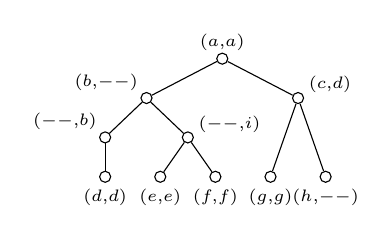
\begin{tikzpicture}[x=.7cm, y=.5cm]
        \node[outside node={below}{(\text{d},\text{d})}] (dd) {};
        \node[outside node={below}{(\text{e},\text{e})}] (ee) at (1, 0) {};
        \node[outside node={below}{(\text{f},\text{f})}] (ff) at (2, 0) {};
        \node[outside node={below}{(\text{g},\text{g})}] (gg) at (3, 0) {};
        \node[outside node={below}{(\text{h},\text{--})}] (h-) at (4, 0) {};
        \node[outside node={120}{(\text{--},\text{b})}] (-b) at (0, 1) {};
        \node[outside node={30}{(\text{--},\text{i})}] (-i) at (1.5, 1) {};
        \node[outside node={120}{(\text{b},\text{--})}] (b-) at (.75, 2) {};
        \node[outside node={30}{(\text{c},\text{d})}] (cd) at (3.5, 2) {};
        \node[outside node={above}{(\text{a},\text{a})}] (aa) at (2.125, 3) {};

        \draw (aa) -- (b-);
        \draw (aa) -- (cd);
        \draw (b-) -- (-b);
        \draw (b-) -- (-i);
        \draw (-b) -- (dd);
        \draw (-i) -- (ee);
        \draw (-i) -- (ff);
        \draw (cd) -- (gg);
        \draw (cd) -- (h-);
    \end{tikzpicture}
    \end{minipage}

    \vspace{.2ex}
    \begin{minipage}[b]{.3\textwidth}\centering\small
        \(S = \text{a(b(def)c(gh))}\)
    \end{minipage}%
    \begin{minipage}[b]{.3\textwidth}\centering\small
        \(T = \text{a(b(d)i(ef)d(g))}\)
    \end{minipage}%
    \begin{minipage}[b]{.4\textwidth}\centering\small
        Alignment of \(S\) with \(T\)
    \end{minipage}
    
    \caption{
        Two hedges \(S\) and \(T\) represented both as terms and as graphs, with a possible alignment of \(S\) with \(T\).
        Both \(S\) and \(T\) are of breadth~1 and degree~3.
        Two hedge intervals are highlighted in blue and green:
        the interval of breadth~2 starting at \enquote{e} in~\(S\)
        and the interval of breadth~1 starting at \enquote{i} in~\(T\).
        \label{fig:hedges}
    }
\end{figure}

Other definitions and results from the previous subsection carry over accordingly, including those of derivations, yield parses, and cyclicity.

\begin{example}[Hedge alignment]\label{ex:for-align}
    The alignment problem on sequences from~\cref{ex:seq-align} can be extended to hedges~\parencite{Jiang1995AlignmentTreesAlternative}.
    An alignment of two hedges \(S\) and \(T\) on \(\Sigma\) is a hedge \(A\) on pairs of \(\Sigma \cup \{\text{---}\}\) such that
    projecting each pair of \(A\) on its first dimension and replacing each node \(\text{---}(h)\) with \(h\) yields \(S\)
    and similarly projecting on the second dimension yields \(T\).
    See \cref{fig:hedges} for an example input and a possible corresponding alignment.

    Once again, the signature for this problem is
    \(\{\algnull, \algplus, \algunit, \algsym{sub}, \algsym{ins}, \algsym{del}\}\).
    However, the \(\algsym{sub}\), \(\algsym{ins}\), and \(\algsym{del}\) operators are binary instead of unary.
    The value \(\algsym{sub}_{\alpha,\beta}(L, R)\) represents an alignment hedge whose first root is a node labeled with \((\alpha,\beta)\) with children \(L\) and siblings \(R\).
    The problem structure is described by the following hedge yield grammar.
    \begin{align*}
        \gramnt{S}[\varepsilon, \varepsilon] &\rightarrow \algunit \\
        \gramnt{S}[\alpha(L)L', \beta(R)R'] &\rightarrow
            \algsym{sub}_{\alpha,\beta}(\gramnt{S}[L, R], \gramnt{S}[L', R']) \\
        \gramnt{S}[LL', \beta(R)R'] &\rightarrow
            \algsym{ins}_{\beta}(\gramnt{S}[L, R], \gramnt{S}[L', R']) \\
        \gramnt{S}[\alpha(L)L', RR'] &\rightarrow
            \algsym{del}_{\alpha}(\gramnt{S}[L, R], \gramnt{S}[L', R'])
    \end{align*}
    For example, a possible derivation to construct the alignment from~\cref{fig:hedges} is
    \begin{align*}
        &\gramnt{S}[\text{a(b(def)c(gh))}, \text{a(b(d)i(ef)d(g))}] \\
        \gramrew\ &\algsym{sub}_{\text{a},\text{a}}(
            \gramnt{S}[\text{b(def)c(gh)}, \text{b(d)i(ef)d(g)}],
            \gramnt{S}[\varepsilon, \varepsilon]
        ) \\
        % \gramrew\ &\algsym{sub}_{\text{a},\text{a}}(
        %     \gramnt{S}[\text{b(def)c(gh)}, \text{b(d)i(ef)d(g)}],
        %     \algunit
        % ) \\
        \gramRew\ &\algsym{sub}_{\text{a},\text{a}}(
            \algsym{del}_{\text{b}}(
                \gramnt{S}[\text{def}, \text{b(d)i(ef)}],
                \gramnt{S}[\text{c(gh)}, \text{d(g)}]
            ),
            \algunit
        )
    \end{align*}
    \begin{align*}
        &\gramnt{S}[\text{def}, \text{b(d)i(ef)}]\\
        \gramrew\ & \algsym{ins}_{\text{b}}(
            \gramnt{S}[\text{d}, \text{d}],
            \gramnt{S}[\text{ef}, \text{i(ef)}]
        ) \\
        \gramrew\ & \algsym{ins}_{\text{b}}(
            \gramnt{S}[\text{d}, \text{d}],
            \algsym{ins}_{\text{i}}(
                \gramnt{S}[\text{ef}, \text{ef}],
                \gramnt{S}[\varepsilon, \varepsilon]
            )
        ) \\
        \gramRew\ & \algsym{ins}_{\text{b}}(
            \algsym{sub}_{\text{d},\text{d}}(\algunit, \algunit),
            \algsym{ins}_{\text{i}}(
                \algsym{sub}_{\text{e},\text{e}}(
                    \algunit,
                    \algsym{sub}_{\text{f},\text{f}}(\algunit, \algunit)
                )
            )
        )
    \end{align*}
    \begin{align*}
        &\gramnt{S}[\text{c(gh)},\text{d(g)}]
        \gramRew \algsym{sub}_{\text{c},\text{d}}(
            \algsym{sub}_{\text{g},\text{g}}(
                \algunit,
                \algsym{del}_{\text{h}}(\algunit, \algunit)
            ),
            \algunit
        ).
        \qedhere
    \end{align*}
\end{example}

Adapting \cref{alg:seq-yield-parser} for hedge patterns results in the following complexity.

\begin{theorem}[Complexity of \cref{alg:seq-yield-parser} on hedges]\label{thm:adp:gram-hedge-complex}
    Let \(\gram\) be a hedge yield grammar of signature~\(\algsign\) and let~\(I\) be a tuple of hedges of size \(n\) and maximum degree \(\deg I\).
    If \(\altrace(\algsign)\) is the trace algebra of \(\algsign\), then \(\Call{\emph{yield-parse}}{\gram, \altrace(\algsign), S, I, \emptyset}\) is an algebraic circuit of size \(\bigo(|P| (n \deg{I})^{\dim \gram})\).
    The algorithm operates in time \(\bigo(|\gram| n^{\dim\gram}(\deg I)^{\dim\gram+\width\gram})\).
\end{theorem}
\begin{proof}
    Each of the up to \(\dim\gram\) arguments of a predicate corresponds to a so-called \emph{hedge interval} of one of the input tapes (see~\cref{fig:hedges}).
    Given a hedge \(h = t_1 \ldots t_k\) of breadth \(k\), a hedge interval of \(h\) is either a subsequence \(t_i \ldots t_j\) where \(1 \le i, j \le k\) (or \(\varepsilon\) if \(i > j\)), or an interval inside one of the trees \(t_i\), i.e., if \(t_i = t(t'_1 \ldots t'_k)\), a hedge interval of  \(t'_1 \ldots t'_k\).
    Each such interval is entirely specified by the root \(v\) of the first subtree included in the interval and by the total number \(d \le \deg I\) of following sibling subtrees included in the interval.
    Hence, there are \(n\deg{I}\) such intervals\footnote{This result was reported by~\textcite{Hochsmann2003LocalSimilarityRNA} who called hedge intervals \emph{closed subforests}.} and the number of entries in \(M\) is \(\bigo(|P| (n\deg{I})^{\dim\gram})\).

    When computing a given table entry, for each clause \(C\), each hedge interval in \(I\) is matched with the corresponding hedge pattern in \(C\) by splitting it into as many hedge subintervals as there are variables in the pattern.
    This decomposition may be performed by recursively walking both the pattern and the input interval and applying the same logic as with sequences when a variable is encountered.
    The total number of split points to consider is at most \(\width\gram\), and each split point is in an interval of length up to \(\deg\gram\), hence the number of decompositions along a given dimension is \(\bigo((\deg I)^{\width\gram})\).
\end{proof}

Following this result, the time complexity from using the hedge yield grammar of~\cref{ex:for-align} is \(\bigo(n^2(\deg I)^3)\) since \(\dim\gram = 2\) and \(\width\gram = 1\).
This bound can be tightened by noticing that, in all cases, at least one of the two dimensions contains a right-maximal hedge interval, i.e., a hedge interval that contains a node followed by all of its siblings.
There are only \(\bigo(n)\) such intervals, as it is not necessary to specify its length.
Hence, the size of the generated circuit stays in \(\bigo(|P|n^2\deg{I})\) and the time complexity is only \(\bigo(n^2(\deg I)^2)\).
This matches the results from~\parencite{Jiang1995AlignmentTreesAlternative}.

% TODO: "Counting, Generating and Sampling Tree Alignments" by Cedric Chauve, Julien Courtiel, Yann Ponty
%   - also gives a way to count tree alignments without ambiguity

% TODO: walking up trees for reconciliation
% Here, we add a third operator, \(A \mid C\), that matches a subtree \(A\) such that \(C\) is its context, i.e., the parent zipper.
% \cite{Huet1997Zipper}
% pointed trees == zipper

% TODO: tree decompositions
%   -> Infrared 2024 <https://link.springer.com/article/10.1186/s13015-024-00258-2>
% feature networks
% > While Infrared proposes a novel form of automated solving of declarative problem specifications by dynamic programming (DP), bioinformatics already has a long tradition of combining declarative methods and dynamic programming in the form of Algebraic Dynamic Programming (ADP) [55]. Despite the common DP backdrop, Infrared and ADP pursue different, even orthogonal goals: instead of deriving a DP algorithm from a declarative problem description, ADP implementations such as GAPC [56] or ADPFusion [57, 58] aim to support the implementation of DP algorithms through algebraic abstraction.

% TODO: word on unordered trees and forests -> NPC problems

\subsubsection{Sets and multisets}

A natural way to decompose sets is through partitions.
A multiset is similar to a sequence but without a specific order on its elements.
Algebraically, they can be seen as sequences but where the concatenation operator is commutative.

\newcommand{\multisets}{\mathcal{M}}

Let \(T\) be a set of terminals. The set \(\multisets(T)\) of \emph{multisets} on \(T\) contains the empty multiset \(\emptyset\) containing no elements, the singleton set \(t\) for \(t \in T\).
For any two multisets \(m\) and \(m'\), \(m\mid m'\) is the multiset containing the elements of \(m\) and the elements of \(m'\).
The multiset addition operator is associative and commutative.

A multiset pattern is an expression that may contain multisets from \(\multisets(T)\) and variables from \(V\) interspersed by multiset additions.
For example \(X \mid Y\) partitions the input multiset into two subsets \(X\) and \(Y\), and \(t \mid X\) extracts an element \(t\) and leaves the remaining elements in \(X\).
The width of a pattern is one less than the number of variables it contains.

% Multiset yield grammars

% Hamiltonian path:
% S[ t | R ] → path_t(S[R])
% S[ t | R ] → S[R]

% Subset sum:
% S[ L | R ] → sum_L

% Set packing:
% S[ x . R, x | E ] → set_x(S[R, E])
% S[ x . R, E ] → S[R, E]
% S[ ε, E ] → 1

Each dimension can hold a subset of one of the input multiset tapes.
There are \(\bigo(2^n)\) such subsets, hence \(\bigo(|P|2^{n\dim\gram})\) table entries.
When matching a multiset with a multiset pattern, this multiset must be partitioned into as many parts as there are variables.
There are \(\bigo((\width\gram + 1)^n)\) such partitions.
Hence the global complexity is \(\bigo(|\gram|2^{n\dim\gram}(\width\gram + 1)^n)\).

This is a slight generalization of the formalism in~\textcite{Siederdissen2015AlgebraicDynamicProgramming} which only considers bipartitions.

Unordered trees and forests can be handled by generalizing multisets to forests in the same way that sequences were generalized to hedges.
The children of a node or the roots in a forest are considered as sets instead of sequences.
In this case, the complexity becomes...

\begin{example}[Unordered forest alignment]\label{ex:for-align-unord}
%
% S[α(L)L', β(R) | R'] → sub(α,β)(S[L, R], S[L', R'])
% S[L | L', β(R)R'] → ...
% S[α(L)L', R | R'] → ...
    A simple modification of~\cref{ex:for-align-unord} gives an algorithm for unordered forest alignment.
    \begin{align*}
        \gramnt{S}[\varepsilon, \varepsilon] &\rightarrow \algunit \\
        \gramnt{S}[\alpha(L)L', \beta(R) \mid R'] &\rightarrow
            \algsym{sub}_{\alpha,\beta}(\gramnt{S}[L, R], \gramnt{S}[L', R']) \\
        \gramnt{S}[L \mid L', \beta(R)R'] &\rightarrow
            \algsym{ins}_{\beta}(\gramnt{S}[L, R], \gramnt{S}[L', R']) \\
        \gramnt{S}[\alpha(L)L', R \mid R'] &\rightarrow
            \algsym{del}_{\alpha}(\gramnt{S}[L, R], \gramnt{S}[L', R'])
    \end{align*}
\end{example}

\subsubsection{Natural numbers}

We consider the decomposition of natural numbers through as sums.
A number expression is either a natural number \(n \in \nat\) or a sum \(n + m\) where \(n\) and \(m\) are two number expressions.
A number pattern is an expression that may contain constant natural numbers and variables from~\(V\).

Each number dimension can hold any value between \(0\) and \(n\), where \(n\) is the value of the initial input.
Note that these values cannot increase above \(n\).
There are \(\bigo(|P|n)\) table entries.
When matching a number with a number pattern, there are %%% multichoice?
possible choices.

\begin{example}[0-1 knapsack]
    Mixes two input tape types, number and sequence.
    \begin{align*}
        \gramnt{S}[N, \varepsilon] &\rightarrow \algunit \\
        \gramnt{S}[N, AR] &\rightarrow \algsym{skip}_A(S[N, R]) \\
        \gramnt{S}[A + N, AR] &\rightarrow \algsym{take}_A(S[N, R]) \\
    \end{align*}
\end{example}

% knapsack
% S[a + B, aR] → take_a(S[B, R])
% S[B, aR] → skip_a(S[B, R])

% eg knapsack, coin change (pseudo-polynomial)
% size of table dimension is O(n), where n is the value of the input (hence exponential)

% number of possible sums
% S[A + B] -> S[A] × S[B]
% S[1] -> unit

% knapsack
% S[I + 1, J] -> S[I, J]
% for each item i: S[i + 1, J + WT[i]] -> S[i, J]
% S[0, J] -> unit
% S[I, 0] -> unit

extend matching to \(A + B\) patterns, where \(A\) and \(B\) sum to the input

\subsubsection{Comparison to other formalisms}

The formalism presented in this subsection is technically less general than the one introduced by \textcite{Berkemer2017AlgebraicDynamicProgramming}.
However, all grammars from their paper can be reframed in the restricted definitions presented here.
In the paper, the hedge intervals are not restricted to intervals on a single level of the input but may span multiple levels.
This increases the complexity as there may be up to \(\bigo(n^2)\) such intervals instead of \(\bigo(n\deg I)\).
It is not clear whether this increased generality is required to solve dynamic programming problems on hedges.

When compared to ICOREs~\parencite{Giegerich2014ModelingDynamicProgramming}, the formalism is also less general.
ICOREs may be converted to yield grammars, however the resulting clauses are not always linear.
The core signature corresponds to our grammar signature.
In an ICORE, a rewrite system is provided for each dimension of the input, and the rules are inverted when compared to the current formalism.
ICOREs use the \(\sim\) symbol to explicitly represent the sequence or hedge concatenation operators, which are implicit here.
Hence, this provides an effective way to parse some ICOREs, which was missing from the literature up to now.
% TODO: do ICOREs always respect linearity?

\subsection{Ambiguity}

Algebraic circuits are called redundant when they encode the same solution multiple times.
While this situation is not problematic when evaluating idempotent algebras, it causes duplicates  and incorrect results when counting or sampling solutions, as discussed in~\cref{sec:adp:space-enum-sample}.
It is therefore desirable to construct yield algebras that produce non-redundant circuits, which we call semantically unambiguous algebras following~\textcite{Reeder2005EffectiveAmbiguityChecking}.

\begin{definition}[Semantic ambiguity]
    A yield grammar \(\gram\) of signature \(\algsign\) is \emph{semantically ambiguous}
    if \(\Call{yield-parse}{\gram, \altrace(\algsign), S, I, \emptyset}\)
    returns a redundant algebraic circuit for some input \(I\).
\end{definition}

This is called \emph{semantic} ambiguity to distinguish it from the usual \emph{syntactic} ambiguity from formal language theory that holds when multiple derivations exist from the same input to different terms.
\textcite{Reeder2005EffectiveAmbiguityChecking} showed that semantic ambiguity, just like syntactic ambiguity, is an undecidable problem.
They also provide heuristics for detecting ambiguity and proof strategies for establishing non-ambiguity.

As pointed out by \citeauthor{Giegerich2000ExplainingControllingAmbiguity}~\cite{Giegerich2000ExplainingControllingAmbiguity}, the encoding of solutions as terms may create opportunities for the same solution to be represented by distinct terms, creating another layer of ambiguity.
For example, under the sequence alignment signature of \cref{ex:seq-align}, the two following terms are distinct \[
    \algsym{sub}_{\text{a},\text{a}}(\algsym{del}_\text{b}(\algsym{ins}_\text{c}(\algsym{sub}_{\text{d},\text{d}}(\algunit))))
    \qquad \algsym{sub}_{\text{a},\text{a}}(\algsym{ins}_\text{c}(\algsym{del}_\text{b}(\algsym{sub}_{\text{d},\text{d}}(\algunit))))
\]
yet they encode structurally identical alignments.
This notion can be made formal through canonicity.

\begin{definition}[Canonical grammars]
    Let \(\algsign\) be a signature and \(k : \alterm(\algsign) \rightarrow K\) be a mapping to a set \(K\).
    A yield grammar of signature \(\algsign\) is \emph{canonical} with respect to \(k\) if it is semantically unambiguous and if, for any input \(I\), there is no repetition among the images of the elements of \(\Call{yield-parse}{\gram, \alterm(\algsign), S, I, \emptyset}\) by \(k\).
\end{definition}

Hence, when analyzing a yield grammar, it is good to reflect on the underlying canonical representation of solutions.
In some cases, the grammar can be modified so as to be canonical.
In the sequence alignment case, intermediate predicates can be used to ensure that insertions always appear before deletions, for example.

Even though canonicity is also undecidable, it can be checked on fixed inputs through classified dynamic programming as in~\cref{ex:classified-algebra}, i.e., by constructing an algebra \(\alclass\) that assigns each term to its class from \(K\) and by running the algorithm on the algebra \(\alclass \times \alcount \mid \alpower \mid \algroup(1)\) and checking if any class has more than one element.

% example: ambiguity in sequence alignment. "standard", "effective" alignments. reference literature on counting alignments
%   - Andrade, H., Area, I., Nieto, J.J., Torres, A.: The number of reduced alignments between two dna sequences (2014)
%  *** - Dress, A., Morgenstern, B., Stoye, J.: The number of standard and of effective multiple alignments. (1998)
%   - Torres, A., Cabada, A., Nieto, J.J.: An exact formula for the number of alignments between two DNA sequences (2003)

% transition:
% non-terminal = predicate = set of ranges inside the sequences
% different predicates ≡ different memoization tables
% predicate dimension ≡ table dimension
% number of variables in predicate argument ≡ number of split points

\subsection{Grammar combinators}


%  - grammar products
%
% given two yield grammars G1 and G2

% direct product: independent dimensions/tapes
%
% predicates take the form (p1, p2) for p1 ∈ P1, p2 ∈ P2
% if p1 has dim l1 and p2 dim l2, then (p1, p2) has dim l1+l2
%
% clauses
% if p1[h1,..,hl1] -> t1 and p2[h'1,..,h'l2] -> t2 are two clauses, create
% (p1, p2)[h1,..,hl1,h'1,..,h'l2] -> ...?

% TODO: how to combine t1 and t2?
% TODO: avoid variables collisions between patterns of p1 and p2
%       (perform α-renaming first)

% single-tape alignment
%
% S[αX] → read_α(S[X])
% S[X] → skip(S[X])
% S[ε] → 1
%
% SS[αX, βY] → read_α(S[X]) read_β(S[Y])
% SS[αX, Y] → read_α(S[X]) S[Y]
%
% t1 = f(A[X], B[Y], C[Z], ...)
% t2 = g(M[F], N[G], ...)
%
% if only one predicate on the rhs
%   fg(AM[X, F])
% otherwise, pair up the predicates? requires same number of predicates in both terms. semantics? cannot repeat a variable in rhs

\cite{Siederdissen2015ProductGrammarsAlignment}

% Does Marchand’s generation of pseudoknot recurrences count as grammar transformations?

Transformations of grammars

\begin{definition}
    Let

    \(A[\alpha_1, \ldots, \alpha_\ell] \rightarrow \)

\end{definition}

\cite{Eisner2016InsideOutsideForward}

% \section{Designing a dynamic programming algorithm}

% summary and "tutorial" part

% \subsection{Inside-outside algorithms}

% - inside/outside algorithm // forward-backward // backprop
%   - differentiation of algebraic circuits (Eisner, Jason 2016)

% «reverse values» -> Joshua Goodman 1999

%%%%%%%%%%%%%%%%%%%%%%%%%%%%%%%%%%%%%%%%%%%%%%%%%%%%%%%%%%%

\section{Conclusion}

Algebraic dynamic programming is based on the central idea that, in dynamic programming algorithms, the descriptions of the solution space structure and of the evaluation schemes for these solutions should be strictly separated.
This allows treating both sides as mathematical objects in their own right.
Many authors have noticed that the evaluation schemes admissible for dynamic programming correspond to algebraic structures called semirings.
In this paper, we presented a unifying formalism that encompasses a sizeable portion of the existing body of literature on such evaluation algebras.
We also presented a set of algebra combinators that may be used to automatically create new algebras from existing ones, generalizing existing similar operators.

As we have noted, the time efficiency of a dynamic programming algorithm is linked to the size of the circuits it produces.
Hence, proving lower bounds on the size of possible circuits generating the solutions to a given problem would yield lower bounds on the time complexity of any dynamic programming solving that problem.
This is the approach taken by~\textcite{Jukna2015LowerBoundsTropical}.
A more general (and probably intractable) problem is that of finding the smallest factorization of a given algebraic circuit.
A systematic solution to this problem could suggest optimizations to existing dynamic programming approaches.
Regarding space complexity, the amount of memory needed for the evaluation of an algebraic circuit corresponds to its pebbling number.
This correspondence underlies the space complexity upper bound of \Cref{lem:algebraic-circuit-eval}.
In general, finding the pebbling number of a circuit is a known PSPACE-complete problem.
But it is still interesting to prove upper bounds for some families of circuits.
Indeed, some unexpected space optimization tricks have been found for some dynamic programming algorithms over the years (see for example Hirschberg’s algorithm for string alignment), and it may be worthwhile to generalize them.

Algebraic dynamic programming has been implemented in multiple systems, most notably 
ADPfusion~\parencite{Siederdissen2012SneakingConcatmap}
and GAP-L~\parencite{Sauthoff2013BellmansGapLanguage}.
Along with this paper, we provide a reference implementation in Python called \emph{padapto} that is aimed primarily at experimentation.

% TODO: connect to
% - Dyna?
% - lower bounds on string alignment
% - min-plus convolution conjecture

% \printbibliography

% \section{Appendix: Other examples}

% \subsection{Travelling salesman}

% \subsection{Phylogenetic reconciliation}

% \subsection{Subset-sum} % or coin-change? (some example on sets)

%%%%%%

% Gotoh algorithm (alignment with affine gaps)
% illustrates multiple non-terminals
% \(\{\algnull, \algplus, \algunit, \algsym{sub}, \algsym{ins-open}, \algsym{ins}, \algsym{del-open}, \algsym{del}\}\)

% {\small\begin{align*}
%     \gramnt{Ed}[\varepsilon, \varepsilon]
%     \rightarrow&\ \algunit \\[1ex]
%     %
%     \gramnt{Ed}[\alpha X, \beta Y]
%     \rightarrow&\ \algsym{sub}_{\alpha, \beta}(\gramnt{Ed}[X, Y]) \\[1ex]
%     %
%     \gramnt{Ed}[X, Y]
%     \rightarrow&\ \algsym{ins-open}(\gramnt{Ins}[X, Y]) \\
%     \gramnt{Ins}[\alpha X, Y]
%     \rightarrow&\ \algsym{ins}_{\alpha}(\gramnt{Ins}[X, Y]) \\
%     \mid&\ \algsym{ins}_{\alpha}(\gramnt{Ed}[X, Y]) \\[1ex]
%     %
%     \gramnt{Ed}[X, Y]
%     \rightarrow&\ \algsym{del-open}(\gramnt{Del}[X, Y]) \\
%     \gramnt{Del}[X, \beta Y]
%     \rightarrow&\ \algsym{del}_{\alpha}(\gramnt{Del}[X, Y]) \\
%     \mid&\ \algsym{del}_{\alpha}(\gramnt{Ed}[X, Y])
% \end{align*}\par}

% \begin{example}[Crossing minimization when drawing two leaf-mapped trees]
%     In this problem, we are given two ordered binary trees with a bijection between their leaves.
%     The goal is to find a way to draw the two trees in the plane without any crossing, and to draw a line segment between each pair of corresponding leaves while minimizing the number of crossings.
%     For a complete treatment of this problem, see~\cite{Fernau2010ComparingTreesCrossing}.
%     Formally, let us denote the two trees \(T\) and \(S\), their sets of leaves as \(L(T)\) and \(L(S)\) respectively, and the bijection \(l : L(T) \rightarrow L(S)\).
%     Find a permutation of the leaves of \(T\) such that, when drawing both trees in the plane and linking each leaf \(v \in L(T)\) to its correspondent \(l(v)\), the number of crossings is minimized.

%     Let us use \(t\) as a binary symbol to denote internal nodes and \(l\) as a nullary symbol to denote leaves.
%     A possible algebra describing the search space is
%     \begin{align*}
%         \gramnt{Cr}[t(T_L, T_R)]
%         \rightarrow&\ \gramnt{Cr}[T_L] \algtimes_{T_L, T_R} \gramnt{Cr}[T_R]
%         \mid \gramnt{Cr}[T_R] \algtimes_{T_R, T_L} \gramnt{Cr}[T_L] \\
%         \gramnt{Cr}[l] \rightarrow&\ \algunit
%     \end{align*}
%     and the following algebra can be used to score the solutions
%     \begin{align*}
%         a \algtimes_{T,T'} b &= a + b + |\{(i, j) \in L(T) \times L(T') \mid l(i) >_S l(j)\}| \\
%         \algunit &= 0
%     \end{align*}
% \end{example}

% S[t(L)|R] → S[L] times_{L,R} S[R]
% S[ε] → 1
